\documentclass[pdftex, 3p, preprint, authoryear, 12pt]{elsarticle}
%\documentclass[16pt]{elsarticle}

\usepackage[utf8]{inputenc}
\usepackage[T1]{fontenc}
\usepackage{geometry}
\geometry{a4paper}
\usepackage[parfill]{parskip}
%\usepackage{ifpdf}
%\renewcommand*\familydefault{\sfdefault} %in stead of cmbright
%\usepackage[cm]{sfmath} %ditto
\usepackage[slantedGreek]{cmbright}
\usepackage{amsmath,esint}
\usepackage{amssymb}
\usepackage{amstext}
\usepackage{upgreek}
\usepackage{ulem}
\normalem
\usepackage{color}
\usepackage{booktabs}
\usepackage{sidecap}
\usepackage[usenames, dvipsnames]{xcolor}
\usepackage{lineno}
\usepackage{imakeidx}
\makeindex
%\usepackage{soul}
\usepackage{soulutf8}
\usepackage{placeins}


\definecolor{newtextcolor}{cmyk}{0.01,0.7,1,0} %% color for new text
\definecolor{newtextcolor2}{cmyk}{1,0.01,0.01,0} %% color for new text
\newcommand{\newtext}[1]{{\color{newtextcolor}#1}}
%\newcommand{\newtextGTE}[1]{{\color{newtextcolor2}#1}}
\newcommand{\BookRef}[1]{{\color{blue}#1}}
\newcommand{\Comment}[1]{{\color{newtextcolor}#1}}
\newcommand{\Figure}[1]{{\color{red}#1}}


%custom color for \hlc
\newcommand{\hlc}[2][yellow]{ {\sethlcolor{#1} \hl{#2}} }
\newcommand{\hlb}[2][blue]{ {\sethlcolor{#1} \hl{#2}} }
\newcommand{\hlr}[2][Maroon]{ {\sethlcolor{#1} \hl{#2}} }
\newcommand{\hlj}[2][OliveGreen]{ {\sethlcolor{#1} \hl{#2}} }
\newcommand{\hlR}[2][red]{ {\sethlcolor{#1} \hl{#2}} }
\newcommand{\hlp}[2][Purple]{ {\sethlcolor{#1} \hl{#2}} }
\newcommand{\hlt}[2][Tealblue]{ {\sethlcolor{#1} \hl{#2}} }


%\newcommand{\ghnote}[1]{{\color{red}#1}}

%boxes and highlight color for text updates, personified!
\newcommand{\ghnote}[1]{\color{white}{\hlb{GH: #1 }}\color{black}}
\newcommand{\ghtxt}[1]{{\color{blue}#1}}
\newcommand{\gtenote}[1]{\color{white}{\hlR{GTE: #1 }}\color{black}}
\newcommand{\gen}[1]{\color{white}{\hlR{GTE: #1 }}\color{black}}
\newcommand{\gtetxt}[1]{{\color{red}#1}}
\newcommand{\gex}[1]{{\color{red}#1}}
\newcommand{\genn}[1]{{\color{orange}#1}}

\newcommand{\tvnnote}[1]{\color{white}{\hlj{TVN: #1 }}\color{black}}
\newcommand{\tvntxt}[1]{{\color{OliveGreen}#1}}

\newcommand{\snnote}[1]{\color{white}{\hlp{SN: #1 }}\color{black}}
\newcommand{\sntxt}[1]{{\color{Purple}#1}}
\newcommand{\slntxt}[1]{{\color{RoyalPurple}#1}}

%\newcommand{\ul}[1]{{\underline{#1}}


\ifpdf
    \usepackage[pdftex,bookmarks=true]{hyperref}
    \hypersetup{
        colorlinks = False,
        linkcolor = blue,
        anchorcolor = blue,
        citecolor = blue,
        filecolor = blue,
        pagecolor = blue,
        urlcolor = blue
    }
\else
    \usepackage[hypertex,bookmarks=true]{hyperref}
        \hypersetup{
        colorlinks = true,
        linkcolor = blue,
        anchorcolor = blue,
        citecolor = blue,
        filecolor = blue,
        pagecolor = blue,
        urlcolor = blue
    }
\fi

\bibliographystyle{plainnat}

\makeatletter
\def\ps@pprintTitle{%
  \let\@oddhead\@empty
  \let\@evenhead\@empty
  \def\@oddfoot{\reset@font\hfil\thepage\hfil}
  \let\@evenfoot\@oddfoot
}
\makeatother

%\journal{...}

%\definecolor{newtextcolor}{cmyk}{0,1,1,0} %% color for new text
%\newcommand{\newtext}[1]{{\color{newtextcolor}#1}}


\begin{document}

%\linenumbers

\begin{frontmatter}

\author{Geir Halnes, Torbjørn V. Ness, Solveig N\ae ss, Klas H. Pettersen, Gaute T. Einevoll}

\title{Book about electrical fields in the brain - \today}

\end{frontmatter}

{\huge Things to consider}
\begin{itemize}

\item Structure plan on: https://www.overleaf.com/2551421161hjxkhwwvjrqk
\item Refer to main Sections as "Chapters", subsections as Sections?
\item When to include functional arguments and not? \gen{Not sure what is meant here.}
\item When to include Units and not? \gen{I think units should be included as much as possible.}
\item How to make this a "computational essay"?
\gen{My thinking is that we should collect all figures with computed examples in the "computational essay" together with a notebook of scripts allowing them to be interactively generated by the reader. 
We should maybe start thinking about what examples to include in what chapter?}
\item Real booky-books tend to have an Index at the end. Add \verb|\index| around words to add them to Index 
\gen{Yes, we should have an index at the end of the book}
\item References after each chapter, or at end of book? \gen{I think at the end of the book.}
\item \gen{It would be good to decide on a rough idea about the length of each of the chapters.}
\item \tvnnote{Kanskje vi bør ha med en enkel oppsummering av elektriske felter også, i et eget kapittel (nytt kapittel 2)? Når man først møter dette fagfeltet kan jo for eksempel linken mellom elektriske ladninger -> elekltriske felter, og elektriske strømmer -> elektriske potensialer være litt forvirrende? Gir også et naturlig sted å snakke om temaer som jording, Maxwell's ligninger etc.?}
\item \tvnnote{Nunez har et eget kapittel med "Fallacies in EEG" med blandt annet seksjonen "Misuse of Physical or Mathematical Models". Vi (mest Gaute kanskje?) kunne kanskje øse litt av vår (mest Gaute sin) erfaring og kunskap med en LFP versjon av dette? Type: sink/source i L4 LFP betyr ikke nødvendigvis at det er L4 celler som lager dette. Unngå strøm-monopoler. Tro på Maxwell's lover. Vær litt forsiktig med Power Laws. Husk at vi oppererer med mange ukjente parametere (elefanten i rommet). osv osv.}
\end{itemize}

\tableofcontents
\newpage
{\huge Part 1}
\section{Introduction} 
\label{sec:Introduction}

\begin{itemize}
\item Why we care \citep{Buzsaki2012,Pettersen2012,Einevoll2013,Einevoll2013a,Einevoll2019}
\end{itemize}


\subsection{Overview of main topics in Part 1}
\ghnote{Vet ikke hvor dette inngaar, men tror det blir fint med et slikt overblikk. Teksten er en skisse.}

\gen{Enig. Kanskje helt til slutt i Part 1, eller helt forst i Part 2? 
"Dette er verkt{\o}yene vi har - now applications ...?"}

We here give a simple overview of what we will deal with in Part 1 of this book by reference to Fig. \ref{fig:Knallfigur}. The extracellular potential largely originates from neuronal transmembrane currents. In the Figure, we have illustrated these for a simple (two-compartment) neuron, with currents that cross its membrane in the form of a current sink $I_1$ in one compartment, and a current source $I_2$ in the other (green arrows). In Chapter \ref{sec:NeuralDynamics}, we describe how to model and compute the intracellular dynamics, the membrane potential dynamics, and the transmembrane currents of neurons (green and yellow arrows). In the following chapters, we shift the focus from neurons to the extracellular medium, where the main focus will be on the extracellular potential $\phi$.

\begin{figure}[!ht]
\begin{center}
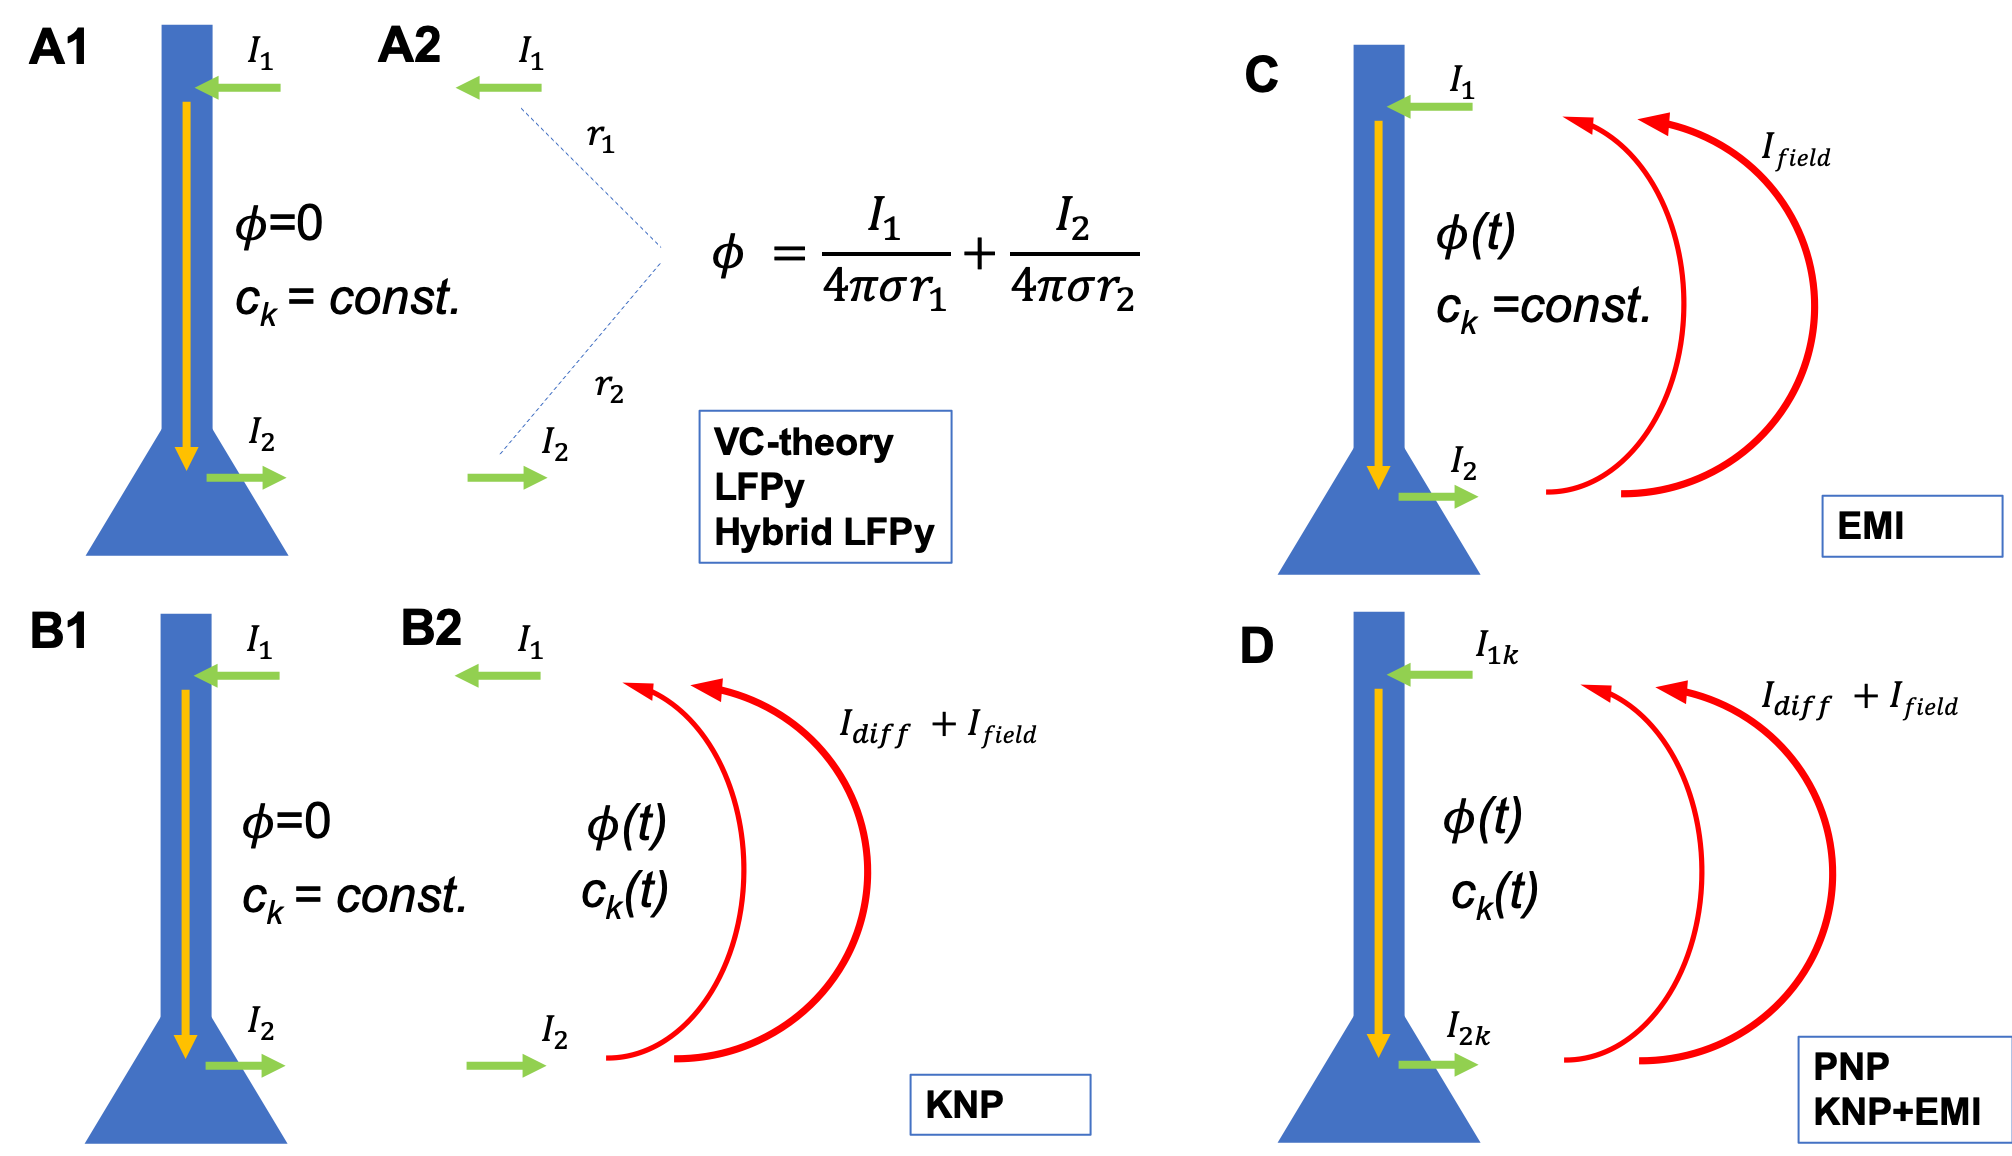
\includegraphics[width=1\textwidth]{Figures/Skjemaoversikt.png}
\end{center}
\caption{\textbf{Overview of the problem that we focus on in this book.} 
}
\label{fig:Knallfigur}
\end{figure}

The simplest take on computing $\phi$ is to treat the extracellular medium as a volume conductor (VC). VC theory then allows us to derive an analytical expression for $\phi$ as a direct function of the neural current sources (Fig. \ref{fig:Knallfigur}A2). Chapter \ref{sec:VC_theory} of this book gives a thorough introduction to VC theory where we derive the key equations from first principles and highlight the many assumptions that the theory is based upon.

A key parameter, and sometimes variable, in VC theory is the conductivity ($\sigma$) of the extracellular medium. In Chapter \ref{sec:conductivity} we give an overview of the experimental and theoretical estimates of $\sigma$. 

Diffusion of ions along extracellular concentration gradients could in principle affect $\phi$. In standard VC theory, such concentrations effects are assumed to be negligible, and ion concentration dynamics is not modeled. This is probably a fairly good approximation for many scenarios, but not for pathological cases, such as epilepsy or spreading depression, which are associated with dramatic concentration shifts in the extracellular medium \cite{Somjen2001, Frohlich2008, Zandt2015review, Ayata2015}. To account for diffusive effects, we need to compute the extracellular dynamics of all individual ion concentrations $c_k$ as well as $\phi$ at all points in space using a suitable numerical electrodiffusive scheme which accounts for diffusion as well as electrical drift og ions (red arrows in Fig. \ref{fig:Knallfigur}B2). In Chapter \ref{sec:eldiff} we present the theory for electrodiffusive processes, and make some estimates of their impact on $\phi$ in different physiological scenarios. 

Another assumption that is typically used when applying VC theory is that the extracellular potential $\phi$ does not have any (ephaptic) effect on the neuronal membrane potential dynamics. This simplifies computations dramatically, because it allows us to perform them in a two-step procedure where we (i) first compute the neurodynamics independently, typically under the assumption that the extracellular potential is zero ($\phi = 0$), and (ii) next use the analytical VC-expression to compute a nonzero $\phi$. The motivation for using this evidently inconsistent approach is that $\phi$ is typically so much smaller than the membrane potential that the ephaptic effects can be neglected without any severe loss in accuracy. This might not be true for all biologically relevant geometries and scenarios, and frameworks that compute the extracellular, membrane and intracellular potentials in a self consistent manner exist (all arrows in Fig. \ref{fig:Knallfigur}C), as do unified frameworks that compute both ion concentrations and electrical potentials in a self consistent manner (all arrows in Fig. \ref{fig:Knallfigur}D). A summary of available frameworks for computing extracellular potentials (and ion concentrations) is given in Chapter \ref{sec:schemes}.

Among the four types of schemes depicted in Fig. \ref{fig:Knallfigur}, the VC scheme is (Fig. \ref{fig:Knallfigur}A) is by far most computationally efficient, as the other schemes require numerical simulations of extracellular dynamics using finite element or finite difference methods. For that reason, the VC scheme is still the gold standard for computing extracellular potentials in large population models of neurons mimicking physiologically realistic scenarios. Therefore, the simulations in the application part of this book (Part 2) will predominantly be based on on standard VC-theory.

\section{Theory: Neural dynamics}
\label{sec:NeuralDynamics}
\begin{itemize}
\item Multicompartmental modeling
\item Cable equation
\item No current monopoles - trick needed for point neurons
\end{itemize}

Modelling of neurons is at the core of computational neuroscience, and the topic has been treated in detail in several text books (see e.g., \cite{KockSegev1998, Koch1999, Hille2001, Dayan2005, Sterratt2011}). We therefore only give a brief introduction to it here. 

\subsection{Multicompartmental modeling}
Most simulations of extracellular potentials are based on multicompartmental neuronal models based on a Hodgkin-Huxley-type formalism. A model of a neuron is then characterized by (i) its morphology, and (ii) its membrane mechanisms. 

In a multicompartmental model\index{multicompartment modelling}, the morphology of the real neuron (Fig. \ref{fig:multicomp}A) is discretized as a set of compartments connected by resistors (Fig. \ref{fig:multicomp}B). In such a model there are two kinds of currents which together determine the membrane potential dynamics of the neuron (Fig. \ref{fig:multicomp}C). These are the currents that run intracellularly between compartments (yellow arrows), and the transmembrane currents (green arrows). Below, first present a framework for modeling the transmembrane currents in a single compartment, and next show how a number of such compartments can be connected together to a multicompartment model.

\begin{figure}[!ht]
\begin{center}
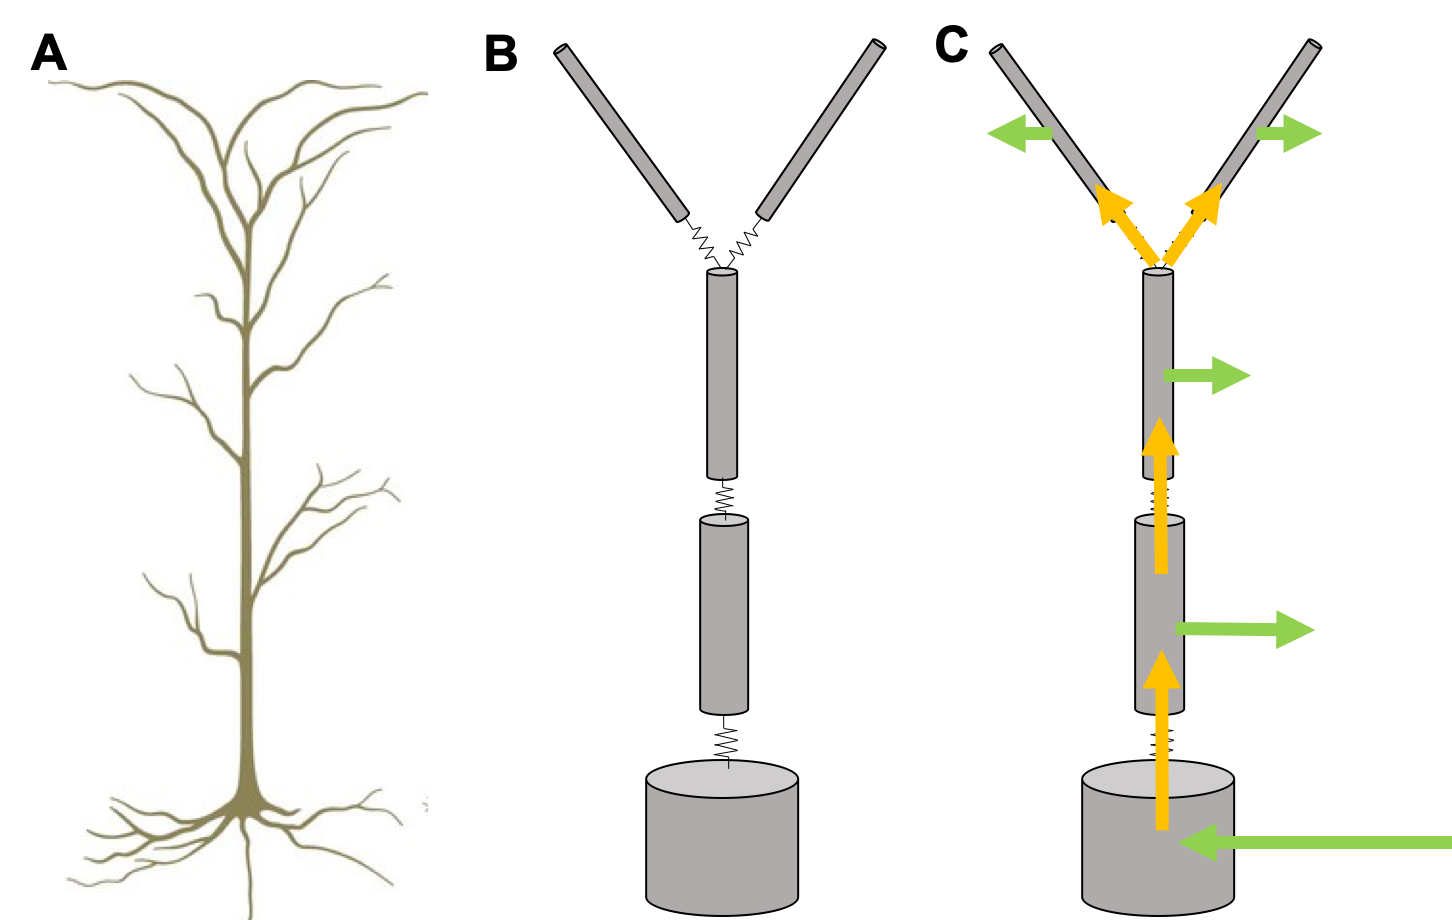
\includegraphics[width=0.6\textwidth]{Figures/Multicomp.png}
\end{center}
\caption{\textbf{Multicompartmental modelling.} 
}
\label{fig:multicomp}
\end{figure}


\subsubsection{Ion channels}
\ghnote{Skriv om HH-formalisme her.}

\subsubsection{Morphology}
\ghnote{Skriv om multicomp her}

\subsection{Cable theory}
\ghnote{Skriv om cable theory her, og noen analytiske tilfeller som hjelper oss aa faa en kjerneforstaaelse.}
\begin{figure}[!ht]
\begin{center}
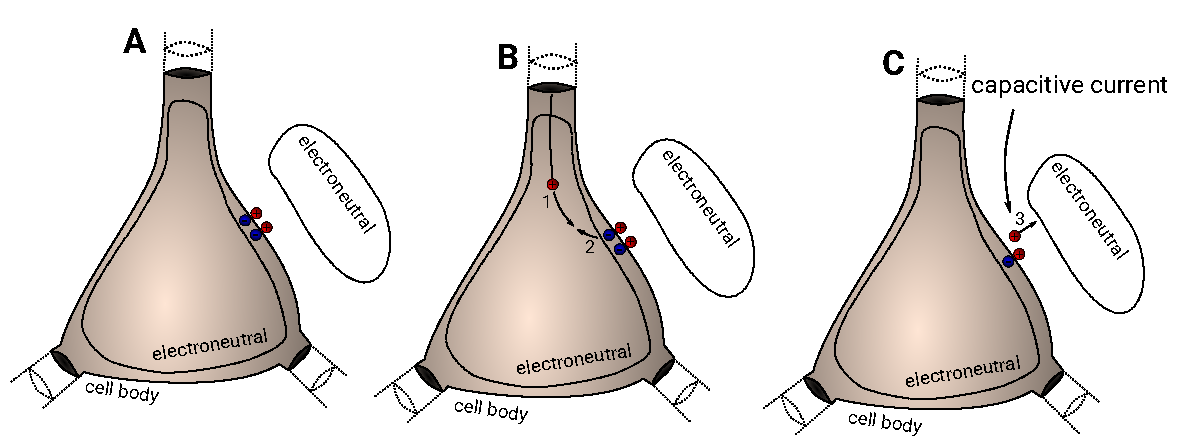
\includegraphics[width=1.0\textwidth]{Figures/capacitive_currents.pdf}
\end{center}
\caption{\textbf{Capacitive currents are important for current conservation} 
\tvnnote{Jeg snek inn denne figuren, så får vi se om vi skal ha den med :-). Det tok en stund før jeg skjønte at kapasitive strømmer er et viktig prinsipp for strømbevaring, så jeg syntes vi burde ha med noe slikt ett eller annet sted.}}
\label{fig:capacitive_currents}
\end{figure}




\subsection{Point neurons}
\ghnote{skriv om punktmodeller her, problemet med at de ikke gir opphav til ekstracellulare felter, og triks for aa bruke dem likevel.}
\tvnnote{Gir det egentlig mening å gå inn på dette før vi har introdusert VC-teori? Hva med å bare kort gå via punktnevroner i utledningen av kabel-ligningen, og henvise til senere seksjoner?}
\subsection{Constant concentrations approximation}
\ghnote{Skrive om konsentrasjonseffekter. Tror det er bra aa spare Nernst-potensialene til dette delkap. Si noe om at man ofte ikke trenger aa holde styr paa konsentrasjoner pga. homeostatiske mekanismer "bakt inn" i passiv lekkasje.Si noe om hva som skal til for faktisk aa modellere konsentrasjoner uten aa gaa inn i detalj. Referere til rammeverkene som kommer i Kap 6.}

\section{Volume conductor theory}
\label{sec:VC_theory}
As we saw in the previous section, simulations of morphologically complex neurons allow us to compute the transmembrane currents entering/leaving the neuron at various locations. This chapter is about how we, when we know the distribution of neuronal current sources, can use volume conductor (VC) theory to predict the extracellular potential at a given point in space. VC theory is the fundament for forward modeling of extracellular potentials at different spatial scales, from extracellular spikes, LFPs and MUAs, to ECoGs and EEGs.

As it used in neuroscience, VC theory rests on a set of assumptions regarding the nature of extracellular current densities ({\bf i}), the medium that they travel through, and the effective conductivity ($\sigma$) for an extracellular current. Instead of introducing these assumptions right away, we start with presenting the VC theory in the form in which it is most commonly used, and postpone a more thorough discussion of the underlying assumptions to the end of the chapter. Before we start deriving the theory, however, we need to make a note on how we approximate the extracellular medium, i.e., the medium that an extracellular current travels through.


%%%%%%%%%%%%%%%%%%%%%%%%%%%%%%%%
\subsection{Continuous, porous medium approximation for VC theory}
\label{sec:continuous}
%%%%%%%%%%%%%%%%%%%%%%%%%%%%%%%%
When presenting the theory for modeling single neurons (Chapter \ref{sec:NeuralDynamics}), we may have given the impression that they are solitary creatures living in a vast extracellular space with long distances to their nearest cell neighbors. This is far from the truth. A cross section of a piece of brain tissue shows that it is densely packed with neural and glial processes (Fig.\ref{fig:ECS}). The extracellular space (colored red in the figure) occupies only about 20 \% of the the total tissue volume. Moreover, it has a highly tortuous geometry, with an average intercell-distance of about 40-60 nm \cite{Sykova2008}. 

\begin{figure}[!ht]
\begin{center}
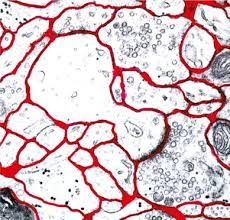
\includegraphics[width=0.3\textwidth]{Figures/ECSdummy.jpeg}
\end{center}
\caption{\textbf{Tortuous medium}  Cross section image of a piece of neural tissue. Extracellular space (marked red) occupies about 20 \% of the total tissue volume, and has a highly tortuous structure. Placeholder, taken from \cite{Sykova2008}.
}
\label{fig:ECS}
\end{figure}

At the microscopic scale, the conductivity $\sigma$ in the brain tissue is thus highly non-homogeneous, as it will be very high at points where there are membranes and much lower in the extracellular space between membranes. Accordingly, electric potentials can vary greatly over tiny distances, and become very large near cell membranes. When we study extracellular potentials, we are typically not interested in these microscopic variations in $\sigma$ and $\phi$, but rather in the values of these entities when averaged over some spatial volume. In practice, the electrodes used in experimental recordings perform such an averaging. Sizes of electrodes used to record extracellular potentials typically range from 5 $\mu$m to 125 $\mu$m in diameter\cite{Viswam2019}, which is larger than the typical diameter of a dendrite ($\sim$ 1 $\mu$m). Experimental recordings thus give us the average potential over a region in space that typically spans over both extracellular space and several neural and glial processes. It is thus the dynamics at this coarse grained spatial scale that we are interested in. 

At the coarse grained spatial scale, it is reasonable to assume that microscale inhomogeneities average out, and that the brain tissue can be treated as a continuous medium \cite{Gratiy2017}. The VC theory presented in this Chapter is based on the continuous medium approximation, and thus describes the extracellular dynamics on a coarse grained spatial scale, with a spatial resolution larger than a micrometer. 

A continuous, porous medium is defined by two key parameters \cite{Nicholson1981}. The first parameter is $\alpha$, is the fraction of the tissue volume that is extracellular space. It typically is about 0.2 in brain tissue, although this can vary between brain regions and even locally due to cellular swelling. The second parameter is $\lambda$, the tortuosity of the medium \cite{Nicholson1981}. It interprets as the ratio between the shortest pathway between two points in space and the euclidian distance between these two points. The tortuosity can be measured experimentally, and for extracellular transport, it has been found that $\lambda = 1.6$ \cite{Nicholson1998}. 

The continuous, tortuous medium approximation has implications for how we interpret the various concepts and variables that we use, so we here give a brief list of definitions: 

\begin{itemize}
\item We will use the term "extracellular medium" to refer to the tissue as it is \textit{experienced} by extracellular currents. It is not the same as the "extracellular solution", i.e. the fluid filling the extracellular space. The extracellular medium is a medium where extracellular currents (i) are confined to move predominantly through the fraction $\alpha$ of the total medium volume, and (ii) must take detours around neural and glial obstacles, as reflected through the tortuosity $\lambda$ \citep{Nicholson1998, Nunez2006}. 

\item  {\bf i} (units $\mathrm{A/m^2}$) will denote the current density for currents traveling extracellularly through the brain tissue. It is defined as current per unit \textit{tissue} (cross-section) area.

\item $\phi$ (unit V) will be used to denote the extracellular potential on the coarse grained scale, i.e., it will represent the extracellular potential averaged over some volume of at least a cube micrometer.

\item $\sigma$ (units S/m) will denote tissue averaged extracellular conductivity, i.e., it is not the (microscopic) conductivity of the extracellular solution, but the coarse-grained conductivity of the extracellular medium as defined above, where the reduced volume fraction and tortuosity are accounted for. Experimental recordings of the extracellular conductivity typically measure 
$\sigma$ as defined in this way. For comparison, the microscopic and unhindered conductivity of the (pure) extracellular solution should theoretically be a fraction $\lambda^2/\alpha$ higher. 

\item $C$ (units A/m$^3$) will denote the current source density (CSD), defined as the local neuronal output current per unit tissue volume.

\end{itemize}

The continuous, porous medium approximation is revisited in Chapter \ref{sec:conductivity}, where we review experimental measurements and theoretical interpretations of the tissue conductivity.


%%%%%%%%%%%%%%%%%%%%%%%%%%%%%%%%
\subsection{From neuronal current sources to extracellular potentials}
\label{sec:continuous}
%%%%%%%%%%%%%%%%%%%%%%%%%%%%%%%%
Throughout this chapter we shall assume that we know the neuronal (and glial) transmembrane currents at all points in space. If they stem from a simulation on a multicompartmental neuron model, they are typically represented as a set of discrete current sources, i.e., one source per neuronal segment (Fig. \ref{fig:CSD}A). As a mathematical generality, we may instead define a continuous density distribution of current sources (Fig. \ref{fig:CSD}B), which we call the current source density ($CSD$). For example, the $CSD$ representing the four point sources in Fig. \ref{fig:CSD}A would be formulated as a sum of four delta functions. 

\begin{figure}[!ht]
\begin{center}
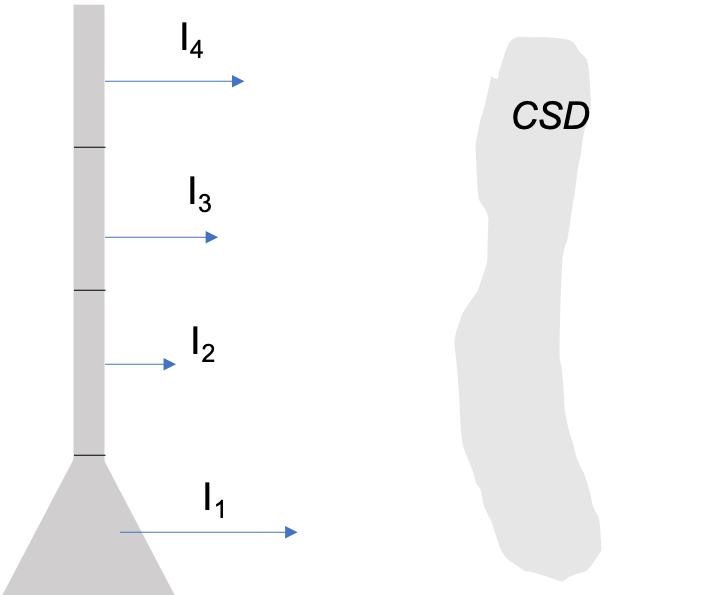
\includegraphics[width=0.3\textwidth]{Figures/CSD.png}
\end{center}
\caption{\textbf{Neuronal current sources.}  {\bf (A)} When simulated on a numerical scheme, the transmembrane currents are known at a discrete set of neuronal segments, i.e., as a set of point sources.  {\bf (B)} As a mathematical generality, we can describe the transmembrane currents as a current source density ($CSD$) distribution. We note the sum of current entering/leaving a neuron is always zero, so that in {\bf (A)}, we must have that $I_1 + I_2 + I_3 + I_4 = 0$, and in {\bf (B)} we have that the spatial integral over the $CSD$ must be zero.
}
\label{fig:CSD}
\end{figure}

Volume conductor theory is essentially based on current continuity in the extracellular medium, i.e., the requirement that no net current can enter/leave a given point in space. Mathematically, current continuity implies that:
\begin{equation}
\nabla \cdot {\bf i}({\bf r}, t) = - CSD({\bf r}, t),
\label{eq:CSD1}
\end{equation}
where ${\bf i}$ is the extracellular current density, and $CSD$ is the current source density. What Eq. \ref{eq:CSD1} essentially tells us, is that if a neuron outputs a current into a (infinitesimal) volume of space (the $CSD$ term), an equally large current leaves that volume as an extracellular current (the $\nabla \cdot {\bf i}$ term).

In this chapter, we shall assume that the extracellular current density is described by:
\begin{equation}
{\bf i}({\bf r}, t) = - \sigma({\bf r}, t) \nabla \phi({\bf r}, t),
\label{eq:ohmici}
\end{equation}
where $\sigma$ is the effective conductivity for an extracellular current in brain tissue. If we combine Eq. \ref{eq:ohmici} and Eq. \ref{eq:CSD1}, we get:

\begin{equation}
\nabla \left( \sigma({\bf r}, t) \nabla \phi({\bf r}, t) \right) = - CSD({\bf r}, t),
\label{eq:CSD2}
\end{equation}

which simplifies to the more commonly used relation:
\begin{equation}
\sigma \nabla^2\phi({\bf r}, t) = - CSD({\bf r}, t),
\label{eq:CSD3}
\end{equation}
in the less general case where the conductivity $\sigma$ is constant. Hence, if we know the distribution of neuronal current sources, we can integrate eq. \ref{eq:CSD2} or eq. \ref{eq:CSD3} to predict the electrical potential in the extracellular space surrounding the sources. 

As indicated above, the variables ${\bf i}$, $\sigma$ and $\phi$ can in general be functions of both position and time. However, for the remainder of this chapter, we shall mostly assume that $\sigma$ is constant. Furthermore, it is implicit in eq. \ref{eq:CSD2} that the relationship between current sources and extracellular potentials is instantaneous (i.e., we can solve eq.  \ref{eq:CSD2} at each time point independently), and in the remainder of the chapter we therefore only use the positional argument for ${\bf i}$ and $\phi$. 

In the following subsections, we show how VC-theory is used to compute $\phi$ in some idealized cases with a homogeneous extracellular medium, and then discuss how this theory can be expanded to more complex cases accounting for inhomogeneities. 


%%%%%%%%%%%%%%%%%%%%%%%%%%%%%%%%
\subsection{Infinite isotropic homogeneous extracellular medium}
\label{sec:isohomo}
%%%%%%%%%%%%%%%%%%%%%%%%%%%%%%%%
We shall now derive an expression for the extracellular potential $\phi$ in the case where the extracellular medium is infinite, isotropic and homogeneous. By homogeneous we mean that the conductivity $\sigma$ is the same everywhere in space, and by isotropic we mean that $\sigma$ is the same in all spatial directions. Although the extracellular medium in reality is neither infinite, nor strictly isotropic and homogeneous, this approximation may still in many cases give fairly good predictions of $\phi$.


%%%%%%%%%%%%%%%%%%%%%%%%%%%%%%%%
\subsubsection{Point source approximation}
%%%%%%%%%%%%%%%%%%%%%%%%%%%%%%%%
We start by deriving the contribution to $\phi$ from a single neuronal point source $I_1$ at the point ${\bf r_1}=0$ (Fig. \ref{fig:pointsource}A). 

\begin{figure}[!ht]
\begin{center}
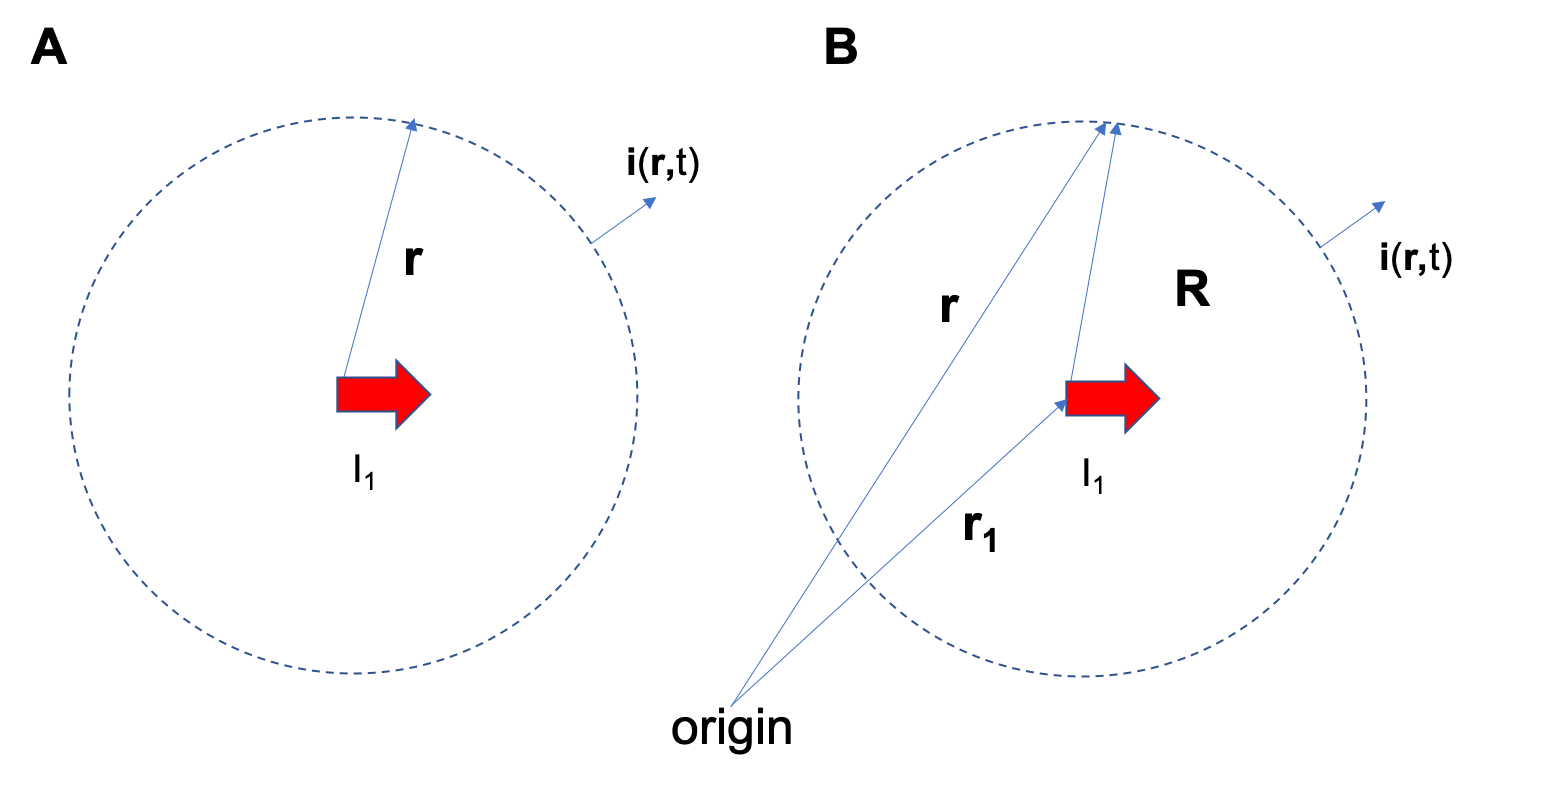
\includegraphics[width=0.6\textwidth]{Figures/Pointsource.png}
\end{center}
\caption{\textbf{Extracellular field from single neuronal point source.} 
}
\label{fig:pointsource}
\end{figure}

Here, we could compute $\phi$ by solving eq. \ref{eq:CSD3}. However, due to the spherical symmetry of this simple case, we can take a shorter path by realizing that the current density (eq. \ref{eq:ohmici}) must radially directed, and that its magnitude must be solely a function of distance $r$ from the source:

\begin{equation}
i({\bf r}) = i(r) = -\sigma \frac{d\phi(r)}{dr}.
\end{equation}

Knowing this, we may find $\phi$ by simply demanding that net current $I_1$ injected into the center of the spherical volume with radius $r$ must equal the net current leaving through the surface of the volume, which in turn must equal the current density $i(r)$ at the surface multiplied with the surface area $4\pi r^2$. We then get the relationship:

\begin{equation}
I_1 = -4\pi \sigma r^2  \frac{d\phi(r)}{dr} \, \iff \, \frac{d\phi(r)}{dr} = -\frac{I_1}{4\pi \sigma r^2 }.
\label{eq:knut}
\end{equation}

To obtain the final solution for $\phi$, we integrate eq. \ref{eq:knut} from $r$ to $\infty$:

\begin{equation}
\int_r^{\infty} \frac{d\phi(r')}{dr'} dr' = \int_r^{\infty} -\frac{I_1}{4\pi \sigma r'^2 } dr'.
\label{eq:knut2}
\end{equation}
Since $\phi({\infty}) = 0$, this leads to the final expression:

\begin{equation}
\phi({\bf r}) = \phi(r) = \frac{I_1}{4\pi \sigma r},
\label{eq:pointsource}
\end{equation}
where $r$ is the distance from the source.

In the above, we made things simple by assuming that the current source was placed in the origin ${\bf r} = 0$. For a point source located in an arbitrary point ${\bf r_1} $, the corresponding expression for the extracellular potential is:

\begin{equation}
\phi({\bf r}) = \frac{I_1}{4\pi \sigma |{\bf r-r_1}|},
\label{eq:pointsource2}
\end{equation}

If we have several point-current sources, $I_{1}, I_2, I_3, ... $ in locations ${\bf r_1}, {\bf r_2}, {\bf r_3} ... $), their contributions add up linearly, and the potential in a point ${\bf r}$ is given by:

\begin{equation}
\phi({\bf r}) = \frac{I_1}{4\pi  \sigma {\bf |r-r_1|}} + \frac{I_2}{4\pi  \sigma {\bf |r-r_2|} } + \frac{I_3}{4\pi  \sigma {\bf |r-r_3|} } + ... = \sum_k \frac{I_k}{4\pi  \sigma {\bf |r-r_k|} }.
\label{eq:pointsources}
\end{equation}


%%%%%%%%%%%%%%%%%%%%%%%%%%%%%%%%
\subsubsection{Line source approximation}
%%%%%%%%%%%%%%%%%%%%%%%%%%%%%%%%
Eq.~\ref{eq:pointsources} is referred to as the point-source approximation \citep{Holt1999, Pettersen2008a}, since it approximates the neuron as a set of point current sources, i.e., the neuron delivers to the extracellular space a singular current source per neuronal segment, located in the segment midpoint. 

A more sophisticated choice may be to assume that the transmembrane current is evenly distributed over the segment axis, choice which is referred to as the line-source approximation \citep{Holt1999, Linden2014}. The contribution to the extracellular potential from a current $I_k$ in a segment $k$ has been found analytically. Here, we skip the derivation, but give the final solution. For a segment with length $\Delta s_k$, the contribution to the extracellular potential will be:

\begin{equation}
\phi({\bf r},t) = \frac{I_k}{4\pi \sigma \Delta s_k} \log \left| \frac{\sqrt{h_k^2+\rho_k^2}-h_k}{\sqrt{l_l^2+\rho_k^2}-l_k} \right|,
\label{eq:linesource}
\end{equation}
Here $\rho_k$ is the distance perpendicular to the line segment, $h_k$ is the longitudinal distance from the end of the segment, and $l_k = \delta s_k + h_k$ is the longitudinal distance from the start of the segment. \ghnote{Burde kanskje ha en figur p{\aa}  dette?}. Eq. \ref{eq:linesource} and Eq. \ref{eq:pointsource} are the equivalent expressions where the transmembrane currents in a single neuronal segment are treated as a line source and point source, respectively. As for the point-source approximation, the contributions from several line-sources add up linearly. That is, if we have multiple segments $k$, the extracellular potential can be computed as:

\begin{equation}
\phi({\bf r},{\bf t}) = \sum_k \frac{I_k}{4\pi \sigma \Delta s_k} \log \left| \frac{\sqrt{h_k^2+\rho_k^2}-h_k}{\sqrt{l_l^2+\rho_k^2}-l_k} \right|,
\label{eq:linesources}
\end{equation}

The line-source approximation is believed to give a better prediction of $\phi$ than the point-source approximation at points in space that are very near neuronal membranes, especially when it comes to predicting rapid fluctuations in $\phi$, such as the extracellular action potential signature \citep{Holt1999}. At points further away from membranes, the two approaches give converging predictions.


%%%%%%%%%%%%%%%%%%%%%%%%%%%%%%%%
\subsubsection{Current source density description}
%%%%%%%%%%%%%%%%%%%%%%%%%%%%%%%%
The forward modelling formulas in Eq. \ref{eq:pointsources} and \label{eq:linesources} can be expressed more generally in terms of the $CSD$. The starting point is then eq. \ref{eq:CSD3}, which for a homogeneous and isotopic medium can be written: 

\begin{equation}
\nabla^2 \phi({\bf r}) = - \frac{CSD({\bf r})}{\sigma}
\label{eq:CSD4}
\end{equation}

Since this is a linear differential equation, we may solve it by first finding its Green's function, i.e., the solution to an impulse response $CSD({\bf r}) = I' \delta^3({\bf r-r'})$, where $\delta^3({\bf r})$ is the Dirac delta function in three dimensions, and $I'$ is the current source at this location. The general solution can then be expressed as a convolution over such Green's functions. Thus, we first seek the solution to: 

\begin{equation}
\nabla^2 \phi({\bf r}) = - \frac{I' \delta^3({\bf r-r'})}{\sigma}.
\label{eq:CSD5}
\end{equation}

We already listed the solution to this in eq. \ref{eq:pointsource2}, but we here provide a more rigorous derivation. We start by by integrating both sides of eq. \ref{eq:CSD5} over an arbitrary 3D volume containing the source:

\begin{equation}
\iiint_V \nabla^2\phi({\bf r}) \,dV =  - \frac{I'}{\sigma} \iiint_V \ \delta^3({\bf r-r'}) \, dV,
\label{eq:marit}
\end{equation}

By the definition of the delta-function, the right hand side of equation \ref{eq:marit} is simply $I'/\sigma$. Using Gauss' theorem, we can convert the volume integral on the left hand side of eq. \ref{eq:marit} to a surface integral, so that eq. \ref{eq:marit} becomes:

\begin{equation}
\oiint_{S} \nabla\phi({\bf r}) \cdot \, d{\bf S}  = - \frac{I'}{\sigma},
\label{eq:berit1}
\end{equation}

To solve this, it is convenient to chose the volume that we integrate over to be a sphere centered at the source location ${\bf r'}$, and with radius $R = |{\bf r-r'}|$ (Fig. \ref{fig:pointsource}B). Due to the symmetry of problem, we then know that the electrical potential is the same for all ${\bf r}$ on the surface of the sphere, so that $\phi({\bf r}) = \phi(R)$. We also know that its gradient $\nabla\phi({\bf r}) = d\phi(R)/dR$ is constant over the surface, and perpendicular to the surface increment $d{\bf S}$. If we use this, eq. \ref{eq:berit1} becomes:
\begin{equation}
\oiint_{S} \frac{d\phi(R)}{dR} d{S}  = - \frac{I'}{\sigma},
\label{eq:berit1ogenhalv}
\end{equation}
which has the solution:
\begin{equation}
4\pi R^2 \frac{d\phi(R)}{dR} = \frac{I'}{\sigma}
\label{eq:berit2}
\end{equation}
If we integrate this from $R$ to $\infty$, and use that $\phi(\infty) = 0$, we get:
\begin{equation}
\phi(R) = \phi({\bf r}) = \frac{I'}{4\pi \sigma R}.
\label{eq:berit3}
\end{equation}
We may now insert back for $\phi(R)= \phi({\bf r})$ and $R = |{\bf r-r'}|$ to obtain the desired Green's function:

\begin{equation}
\phi({\bf r})= \frac{I'}{4\pi \sigma |{\bf r-r'}|},
\label{eq:berit4}
\end{equation}
As earlier stated, the solution for a general $CSD$ can be expressed as a convolution over the Green's function, so that:

\begin{equation}
\phi({\bf r}) = \frac{1}{4\pi \sigma}\iiint_V \frac{CSD({\bf r'})}{|{\bf r}-{\bf r'}|} \,dV, 
\label{eq:csds}
\end{equation}
where the volume integral runs over all sources. Here, the $CSD$ represents whatever approximation one used for the current sources, and eq. \ref{eq:csds} is the continuous counterpart to eq. \ref{eq:pointsources}. If we describe the CSD as a sum of point sources, i.e.,  $CSD({\bf r}) = \sum_k I_k \delta^3({\bf r} - {\bf r_k})$, eq. \ref{eq:csds} reduces to eq.\ref{eq:pointsources}.



%%%%%%%%%%%%%%%%%%%%%%%%%%%%%%%%
\subsection{Infinite anisotropic homogeneous extracellular medium}
\label{sec:anisohomo}
%%%%%%%%%%%%%%%%%%%%%%%%%%%%%%%%
In the previous subsection we assumed that the extracellular conductivity $\sigma$ was the same in all spatial directions. It is relatively straightforward to expand the VC theory to the case of an anistotropic $\sigma$. If we use the point source approximation, and denote the conductivity in the different spatial directions $\sigma_x$, $\sigma_y$ and $\sigma_z$, the extracellular potential surrounding a set of point current sources $I_k$ is given by \citep{nicholson1975, Pettersen2012}:

\begin{equation}
\phi(x,y,z) = \sum_k \frac{I_k}{4\pi(\sigma_y\sigma_z (x-x_k)^2 + \sigma_x\sigma_z (y-y_k)^2 + \sigma_x\sigma_y (z-z_k)^2)}.
\label{eq:Panisos}
\end{equation}
If we use the CSD-description of the sources, the corresponding expression is:

\begin{equation}
\phi(x,y,z) = \iiint_V \frac{CSD(x,y,z)}{4\pi(\sigma_y\sigma_z (x-x_k)^2 + \sigma_x\sigma_z (y-y_k)^2 + \sigma_x\sigma_y (z-z_k)^2)} \, dV, 
\label{eq:Canisos}
\end{equation}

In general, the brain does not have an isotropic $\sigma$. For example, in cortex it has been found that the conductivity is about 50\% higher in the depth direction, i.e., for currents running in parallel to the axis of pyramidal cell dendrites \citep{Goto2010}. However, the overall effect of the anisotropy on extracellular potentials often appears to be quite weak \citep{Ness2015}, and the approximation that $\sigma$ is isotropic often gives good predictions of the potential.


%%%%%%%%%%%%%%%%%%%%%%%%%%%%%%%%
\subsection{Nonhomogeneous extracellular medium}
\label{sec:nonhomo}
%%%%%%%%%%%%%%%%%%%%%%%%%%%%%%%%
\ghnote{Enter Torbj{\o}rn}. 

\begin{itemize}
\item Method of Images \citep{Ness2015}
\item FEM \citep{Ness2015}, ...
\end{itemize}


\subsection{Modelling the electrode}
\label{sec:electrode}
\begin{itemize}
\item Disc-electrode approximation
\end{itemize}
\ghnote{Enter Torbj{\o}rn: Tekst her klippet fra bokkapittelet:}. 

The simplest and most commonly used approach when modeling extracellular recordings is to calculate the extracellular potential at single points following one of the approaches outlined above, and use this as a measure of recorded potentials. Implicitly, this assumes ideal point electrodes, that is, the electrodes (and electrode shank) do not affect the extracellular potential and the extracellular potential does not vary substantially over the surface of the electrodes. (The point-electrode assumption was used for all simulation examples in this chapter).

A numerically straightforward extension is the disc-electrode approximation where the potential is evaluated at a number of points on the electrode surface, and the average calculated \citep{ Linden2014}. 
This approach takes into account the physical extent of the electrode, but not any effect the electrode itself might have on the electric potential. 
Close to the electrode surface the electric potential will however be affected by the presence of the high-conductivity electrode contact \citep{McIntyre2001, Moulin2008}. A numerically much more comprehensive approach to modeling electrodes is to use the Finite Element Method (FEM) to model the electrode \citep{Moulin2008, Ness2015}, or the electrode shank \citep{Moffitt2005, Buccino2019b}. Using FEM for validation, \cite{Ness2015} found that the ideal point-electrode and disc-electrode approximations where reasonably accurate when the distance between the current sources and the recording electrode was bigger than $\sim$4 times and $\sim$2 times the electrode radius, respectively, indicating that the effects of the electrodes themselves are negligible in most cases \citep{Nelson2010}.
The presence of large multi-contact electrode probes can, however, substantially affect the extracellular potential in its vicinity, by effectively introducing a large non-conducting volume~\citep{Mechler2012}, and this can amplify or dampen recorded potentials from nearby cells by almost a factor of two, depending on whether the cell is in front of or behind the electrode shank \citep{Buccino2019b}.

Note that for modelling current stimulation electrodes (as opposed to just recording electrodes), more complex electrode models might be needed due to electrode polarization effects \citep{McIntyre2001, Martinsen2008, Joucla2012}.


%%%%%%%%%%%%%%%%%%%%%%%%%%%%%%%%
\subsection{Dipole approximation}
\label{sec:dipole}
%%%%%%%%%%%%%%%%%%%%%%%%%%%%%%%%
\ghnote{Enter Solveig}

By reformulating Eq.~\eqref{eq:VCtheory}, we find that the electric potential from a volume containing a combination of current sinks and sources, can be precisely described by the multipole expansion \citep{Nunez2006}:

\begin{equation}\label{eq:multipole}
\Phi(R) = \frac{C_{monopole}}{R} + \frac{C_{dipole}}{R^2} + \frac{C_{quadrupole}}{R^3} + \frac{C_{octupole}}{R^4} + ...
\end{equation}
when the distance from the center of the volume to the measurement point is larger than the maximal distance from volume center to source [cite - find Jackson!].

In neural tissue, current monopoles are unphysical due to current conservation and the quadrupole, octopole and higher-order contributions decay rapidly with distance $R$. Consequently, the multipole expansion can be approximated by the dipole contribution for large distances, a simplification known as the current dipole approximation \citep{Nunez2006}:
\begin{equation}\label{eq:CDA}
\Phi(\mathbf{R}) \approx \frac{1}{4 \pi \sigma} \frac{|\mathbf{p}| \cos \theta}{R^2}.
\end{equation}
Here, $\mathbf{p}$ is the current dipole moment and $\theta$ is the angle between the current dipole moment and the distance vector $\mathbf{R}$. The current dipole moment can be found by summing up all the transmembrane currents from a neuron \citep{Pettersen2008, Pettersen2014, Nunez2006}: 
\begin{equation}\label{eq:dipole}
\mathbf{p} = \sum_{k=1}^N I_k \mathbf{r}_k.
\end{equation}
For a current sink $-I$ at location $\mathbf{r}_1$ and a current source $I$ at location $\mathbf{r}_2$, the current dipole moment can be formulated as $\mathbf{p} = -I\mathbf{r}_1 + I\mathbf{r}_2 = I(\mathbf{r}_2 - \mathbf{r}_1) = I\mathbf{d}$, where $\mathbf{d}$ is the distance vector between the current sink and the current source, giving the length $d$ and direction of the current dipole. As mentioned above, the current dipole approximation is applicable when we are in the far-field limit, that is when $R$ is much larger than the dipole length: $R > 3d$ or $R > 4d$ \citep{Nunez2006}.

The point-source approximation, Eq. \ref{eq:VCtheory} (or the line-source version of it), and the current dipole approximation, Eq.~\eqref{eq:CDA} represent volume conductor theory in its simplest form, and are based on a set of assumptions, some of which may be relaxed for problems where it is relevant: 


%%%%%%%%%%%%%%%%%%%%%%%%%%%%%%%%
\subsection{Approximations used in VC theory}
\label{sec:approximations}
%%%%%%%%%%%%%%%%%%%%%%%%%%%%%%%%
The VC theory presented in this Chapter relies on several assumptions and approximations. Below, we discuss the most important of these. 

\subsubsection{Quasi-static approximation of Maxwell's equations}
\label{sec:quasistatic}
In the quasi-static approximation to Maxwell's equations, one neglects terms with the time derivatives of the electric and magnetic fields. For linear materials with instantaneous response properties, Maxwell's (macroscopic) equations for the curl of the electric and magnetic fields can then be simplified to:
\begin{equation}
\nabla \times {\bf E} = - \frac{\partial {\bf B}}{\partial t}  \approx 0, 
\label{eq:maxE}
\end{equation}
and
\begin{equation}
\nabla \times {\bf B} = \mu{\bf i} + \mu \epsilon \frac{\partial {\bf E}}{\partial t} \approx  \mu {\bf i} ,
\label{eq:maxB}
\end{equation}
where $\mu$ and $\epsilon$ are the permeability and permittivity of the medium respectively. It follows from eq. \ref{eq:maxE} that the static electric field is conservative, and related to an extracellular potential through,
\begin{equation}
{\bf E} = \nabla \cdot \phi.
\label{eq:conservative}
\end{equation}
The quasi-static approximation appears to be well-justified for the relatively low frequencies relevant for brain signals, below about 10 kHz \cite{Nunez2006, Grodzinsky2011}.


\subsubsection{Linear extracellular medium} 
In a linear extracellular medium, the relationship between the current density and the electrical field is given by
\begin{equation}
{\bf i} = \sigma {\bf E}.
\label{eq:bertil}
\end{equation}
This relation is constitutive, meaning that it is observed in nature rather than derived from any physical principle \citep{Nunez2006, Pettersen2012}. It is quite general, and $\sigma$ can here in principle be anisotropic (i.e., a tensor, accounting for different conductivities in different directions), inhomogeneous (position dependent), and complex (accounting for capacitive effects). We note that eq. \ref{eq:bertil} is generally only valid in the frequency domain, while in the time domain, ${\bf i}$ must be given as a temporal convolution of $\sigma$ and ${\bf E}$ \cite{Bedard2009}. However, if $\sigma$ is frequency independent (this assumption is discussed further below), eq. \ref{eq:bertil} will also be valid in the time domain.

Eq. \ref{eq:bertil} is essentially Ohm's law for a volume conductor. If we combine it with 
the quasi-static approximation (i.e., with eq. \ref{eq:conservative}), we get a current density given by ${\bf i} = \sigma \nabla \phi$, which is what we assumed in the beginning of this chapter (eq. \ref{eq:ohmici}).


\subsubsection{Extracellular currents are exclusively due to Ohmic drift} 
\label{sec:onlyohmic}
When basing the VC theory on eq. \ref{eq:ohmici}, we assumed that extracellular currents are mediated exclusively by Ohmic drift. In principle, the extracellular current density could have additional contributions from diffusion of ions, advection currents and displacement currents:

\begin{equation}
{\bf i} = {\bf i^{ohm}} + {\bf i^{dif}} + {\bf i^{adv}} + {\bf i^{dis}}, 
\label{eq:generalcurrent}
\end{equation}

The advective current, 
\begin{equation}
{\bf i^{adv}} = F \rho {\bf u}, 
\label{eq:iadv}
\end{equation}
is the current that arises in a bulk solution if the solution has a charge density $\rho$ that it drags along with it due to a bulk flow with velocity ${\bf u}$, while the displacement current,
\begin{equation}
{\bf i^{dis}} = \frac{\partial \rho}{\partial t},
\label{eq:idis}
\end{equation}
represents the capacitive effect of a medium that allows local charge accumulation, so that $\rho$ can vary with time.  

For the physiological conditions of the extracellular solution, the charge relaxation time, i.e., the time it takes for $d\rho/dt$ to decay to zero when responding to a change in the electric field, is in the order of 1 ns \cite{Grodzinsky2011, Gratiy2017}. This means that the displacement current (eq. \ref{eq:idis}) will mainly be important under conditions when the electrical field varies with frequencies in the GHz range. As the relevant fields with physiological origin vary with frequencies that are orders of magnitude lower than this, the displacement current can safely be neglected. Related to this, the actual charge accumulation that takes place during a relaxation time of 1 ns is very small. For most practical purposes it is a therefore good approximation to assume that the extracellular medium is electroneutral \cite{Solbra2018}, which means that $\rho = 0$ so that the advective current becomes zero. Hence, for practical purposes, it is safe to assume that both the displacement current (eq. \ref{eq:idis}) and the advective current (eq. \ref{eq:iadv}) give negligible contributions to extracellular dynamics. A more physically rigorous argument for this was given in \cite{Gratiy2017}. 

The diffusive current,
\begin{equation}
{\bf i^{dif}} = -F \sum_k z_k D_k \nabla c_k,
\label{eq:idif}
\end{equation}
represents the current that arrises when ions (with valence $z_k$ and diffusion constants $D_k$) diffuse along extracellular concentration gradients ($\nabla c_k$), and carry along with them a net charge. Diffusive currents are neglected in standard VC theory under the assumption that they are much smaller than Ohmic drift currents at the coarse grained scale of brain tissue. By estimates, the effect of diffusion on $\phi$ is most likely small under normal conditions, 
so that one might generally make quite good predictions with a VC theory that neglects them \cite{Halnes2016, Gratiy2017}. 
However, diffusive currents can have a notable impact on $\phi$ in physiological conditions with large concentration gradients \cite{Halnes2016, Gratiy2017}. Diffusive effects on $\phi$may therefore be particularly relevant under pathological conditions such as epilepsy, stroke and spreading depression, which are associated with dramatic shifts in local extracellular concentrations (see e.g.,  \cite{Somjen2001, Frohlich2008, Wei2014, Ayata2015}). 

To account for diffusive effects, one needs to compute not only the electrical potential, but also the ion concentration dynamics of all involved ions at all points in space. This can not be done using VC theory in the standard form presented here, but can be done using Finite Element Methods \cite{Solbra2018}. We go through the theory for modelling electrodiffusive systems in Chapter \ref{sec:eldiff}.


\subsubsection{Frequency independent conductivity} 
\label{sec:f-independent}
Generally, the response of a medium to an imposed alternating current can depend on the frequency of the current. Then, the conductivity contains a resistive part, which is real and frequency independent, and an imaginary part that account for capacitive and inductive effects that are frequency dependent. Above (Chapter \ref{sec:onlyohmic}) we argued that the extracellular displacement current is negligible, which means that the extracellular medium in itself does not exhibit any capacitive effects. This alone does not rule out the possibility that the effective conductivity of the tissue medium includes capacitive effects, as an extracellular current traveling through it could interact with nearby capacitive neural membranes. However, for the relevant frequencies in extracellular recordings, the capacitive and inductive effects appear to be negligible compared to the resistive effects \cite{Logothetis2007, Miceli2017, Ranta2017}. We have therefore based the VC theory presented here on the assumption that the medium is Ohmic or resistive, meaning that we the imaginary and frequency dependent part of the conductivity is zero. We note, however, that it is possible to expand the formalism to include a frequency dependent conductivity \cite{Bedard2004, Tracey2011, Miceli2017}. 


\subsubsection{Isotropic conductivity} 
A commonly used approximation in VC theory, is that $\sigma$ is isotropic, i.e., the same in all spatial directions. This is mostly an acceptable approximation, and the theory presented in Section \ref{sec:isohomo} relied on this assumption. However, as we showed in Section \ref{sec:anisohomo}, it is possible to expand the formalism to account for an anisotropic conductivities.


\subsubsection{Homogeneous conductivity} 
Another commonly applied assumption in VC theory, is that the conductivity is the same everywhere, an assumption that we used in Section \ref{sec:isohomo} and Section \ref{sec:anisohomo}, but relaxed in Section \label{sec:nonhomo}. Clearly, this assumption does not hold on the micrometer scale, where neural tissue is highly non-homogeneous \citep{Nicholson1998}. However, microscale inhomogeneities tend to average out on a larger spatial scale (cf. the continuous medium approximation), and a homogeneous conductivity appears to be a reasonable approximation, at least within a given brain region such as cortex \citep{Logothetis2007}. 

When signals are recorded very far from their sources, it is likely that they on their journey have experienced a $\sigma$ that varied on a macroscopic scale. For example, the signals recorded in the EEG have traveled through both brain tissue, bone and skin, which are three different media with different conductivities. When $\sigma$ is non-homogeneos, there is no general analytical formula available (like eqs. \ref{eq:csds} or \ref{eq:anisos}) that link the extracellular potentials to the underlying current sources. Analytical solutions can still be obtained for some simple non-homogeneous cases, such as those presented in Section \ref{sec:nonhomo}. For more general cases, one can in principle always solve eq. \ref{eq:CSD2} for arbitrarily complex geometries with varying conductivities using numerical methods, like the Finite Element Method (FEM) \citep{Logg2012}. For examples of neuroscience applications using this approach, see \cite{Moffitt2005, Frey2009, Joucla2012, Haufe2015, Ness2015, Buccino2019b, Obien2019}. 

\ghnote{Noe av dette kan kanskje flyttes til Torbjorns kapittel.}




\subsubsection{No ephaptic coupling} 
Ephaptic coupling refers to the effect where the activity of a neuron affects the membrane potential of another neuron or itself through the extracellular potential it creates. The VC theory presented here does not in itself make any assumption regarding ephaptic effects being present or not. That is, eq. \ref{eq:csds} for the extracellular potential holds regardless of whether the or not ephaptic effects were accounted for when the neurodynamics, i.e., the $CSD$ was computed. However, in the practical usage of the VC theory, ephaptic effects are typically neglected since it makes things a lot simpler to do so. Then, neurodynamics and extracellular potentials can be computed in two independent steps. That is, first the neuronal transmembrane currents are computed under the assumption that the extracellular potential is zero (cf. Chapter \ref{sec:NeuralDynamics}), and next, the computed transmembrane currents are used to predict a non-zero extracellular potential (cf. eg. \ref{eq:csds}). Despite its evident inconsistency, this approach can give fairly accurate results since extracellular potentials are generally so much smaller than the membrane potential that the ephaptic effect is small. There are, however, aspects of neuronal activity that can not be understood without accounting for ephaptic effects \cite{Holt1999, Anastassiou2015, Goldwyn2016}. 

To account for ephaptic effects, one must model the neurodynamics and extracellular potential simultaneously on a unified framework, which is more computationally challenging (more on this in Chapter \ref{sec:schemes}).




\section{Extracellular conductivity}
\label{sec:conductivity}
\index{Extracellular conductivity}

\begin{itemize}
\item Experimental measurements \citep{Miceli2017}
\item Theoretical explorations \citep{Meffin2012,Tahayori2012,Meffin2014,Tahayori2014}
\end{itemize}

\begin{figure}[!ht]
\begin{center}
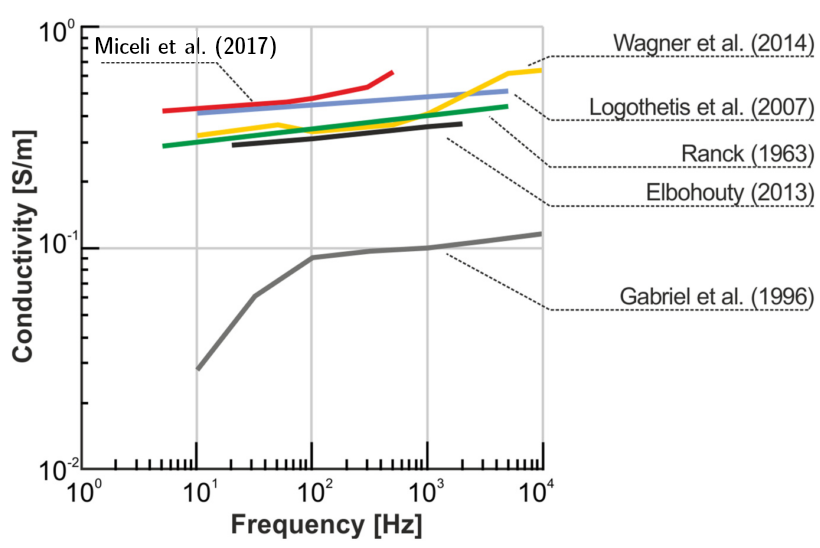
\includegraphics[width=0.6\textwidth]{Figures/Sigma/frequency_dependence.png}
\end{center}
\caption{\textbf{Literature review of reported conductivities in various species and experimental setups.} 
Most studies seem to indicate a very weak frequency dependence of the extracellular conductivity\index{conductivity}, which would have a negligible effect on measured extracellular potentials \citep{Miceli2017}. The very low and strongly frequency dependent values measured by \cite{Gabriel1996} represents an outlier, and although it has received substantial attention, it has to the best of our knowledge not been reproduced by any other study.
For details about the data, see \cite{Miceli2017}, and references therein \citep{Ranck1963, Gabriel1996, Logothetis2007, Elbohouty2013, Wagner2014}
}
\label{Sigma:fig:freq_dep}
\end{figure}


\begin{figure}[!ht]
\begin{center}
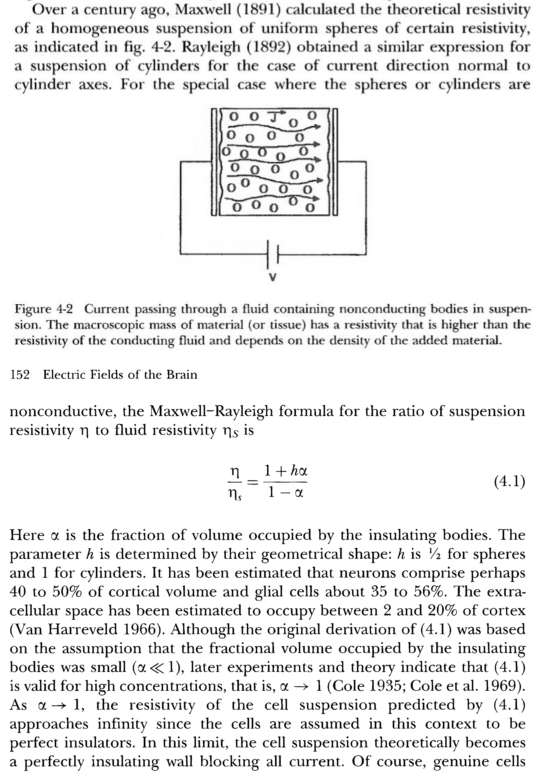
\includegraphics[width=0.6\textwidth]{Figures/Sigma/resistivity_maxwell.png}
\end{center}
\caption{\textbf{From Nunez} \tvnnote{Ta med noe slikt?}}
\label{Sigma:fig:maxwell_resistivity}
\end{figure}

\subsection{Capacitive effects in neuronal tissue}
At high frequencies, extracellular currents could pass through neurons as capacitive currents.
\tvnnote{Utledning tilsvarende Appendix B i Nunez?}
\section{Electrodiffusion in the extracellular space}
\label{sec:eldiff}
In the standard VC theory presented in Chapter \ref{sec:VC_theory}), we assumed that extracellular currents, and thus extracellular potentials, are exclusively due to ohmic drift. However, when ion concentrations are present in the extracellular space, there will also be diffusive currents present, which can evoke so called diffusion potentials. 

In this chapter, we will introduce a more general, electrodiffusive theory for extracellular dynamics, which accounts effects of ionic diffusion as well as ohmic drift. However, before we present the electrodiffusive theory, we will try to get an intuition of how diffusion potentials arise.

\subsection{What is a diffusion potential?}
To get a qualitative understanding of what a diffusion potential is, let us consider a simple two-compartment system with two ionic solutions interacting at a junction  (Fig. \ref{Eldiff:fig:diffpot}). We assume that we in one compartment (the left) have a high concentration of NaCl, and in the other compartment (the right) have a lower concentration of NaCl (Fig. \ref{Eldiff:fig:diffpot}A). Initially, both compartments are electroneutral, i.e., they contain equal amounts of Na$^+$ and Cl$^-$. As there are no electrical forces present, the initial system dynamics will be driven exclusively by diffusion. 

\begin{figure}[!ht]
\begin{center}
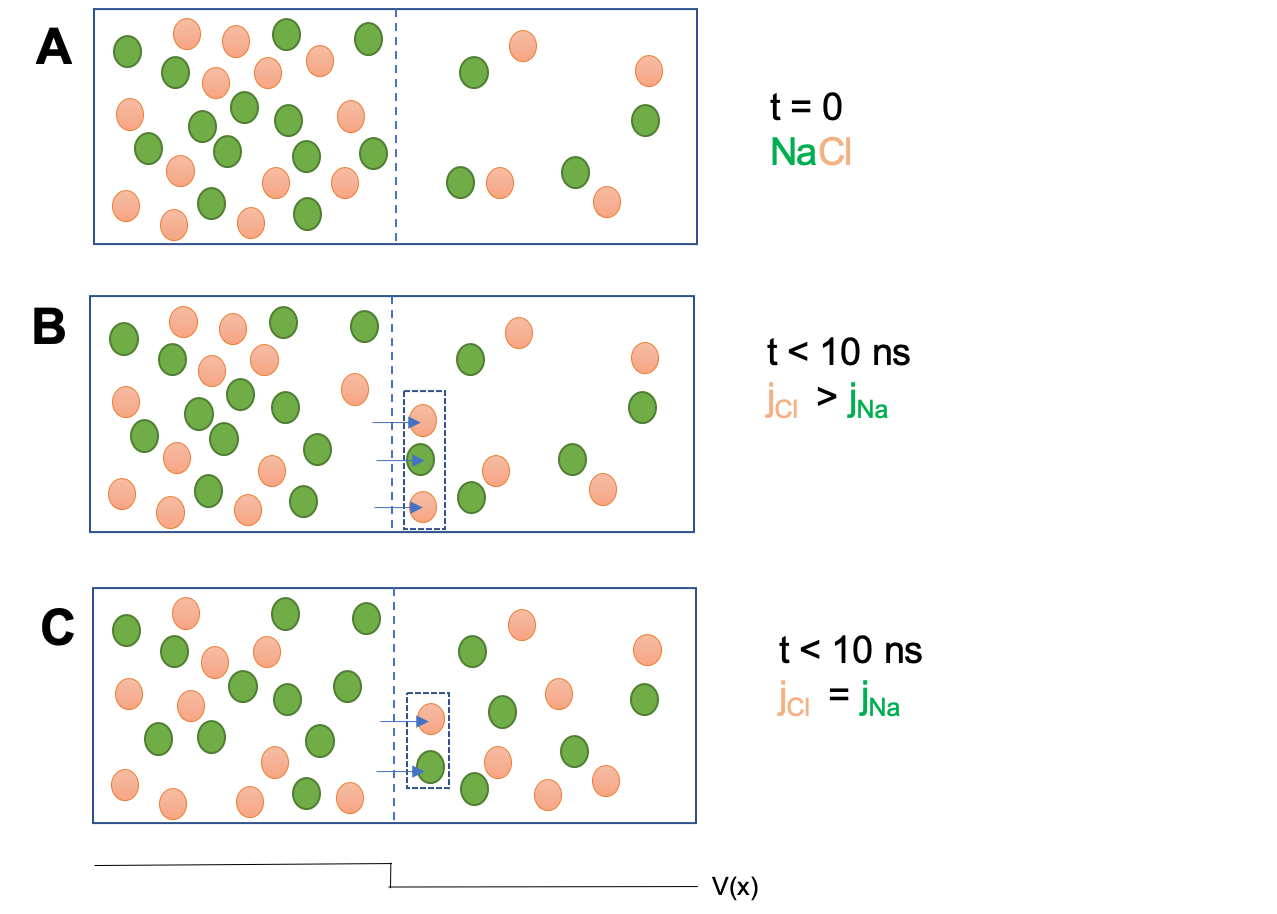
\includegraphics[width=0.8\textwidth]{Figures/Eldiff/Diffusionpot.png}
\end{center}
\caption{\textbf{Diffusion potential at the junction between two ionic solutions}. ({\bf A}) Initial condition with high concentration NaCl in the left compartment and low concentration NaCl in the right compartment. ({\bf B}) Since $D_{Cl} > D_{Na}$, we initially expect the flux of Cl$^-$ to be higher than the flux of Na$^+$. ({\bf C}) The net charge transfer in ({\bf B}) will give rise to a potential difference $\phi_d$ between the two compartments, which will prevent further charge accumulation. }
\label{Eldiff:fig:diffpot}
\end{figure}

Without solving any equations, we intuitively realize that initially, both Na$^+$ and Cl$^-$ will diffuse towards the low-concentration compartment on the right-hand-side. The diffusion speed for the various ions will be proportional to their respective diffusion constants, which in dilute solutions have the values given in Table \ref{tab:diffconsts}). As the Table shows, the diffusion constant for Cl$^-$, is higher than that for Na$^+$. This means that rightward diffusive flux of Cl$^-$ will initially be larger than that for Na$^+$  (Fig. \ref{Eldiff:fig:diffpot}B). 

\begin{table}[h!]
\begin{center}
\caption{Diffusion constants}
\label{tab:diffconsts}
    \begin{tabular}{l|l}
    \hline
    $D_{Na}$ & $1.33\times 10^{-9}$ m$^2$/s\\ \hline
    $D_K$ & $1.96  \times 10^{-9}$ m$^2$/s \\ \hline
    $D_{Cl}$ & $2.03 \times 10^{-9}$ m$^2$/s \\ \hline
    $D_{Ca}$ & $0.71\times 10^{-9}$ m$^2$/s \\ \hline
    \end{tabular}
\end{center}
\end{table}

The fact that we initially have a higher flux of anions than of cations is quite dramatic. A charge-separation process like that will lead to an accumulation of positive charge in the left compartment and negative charge in the right compartment. In turn, this will lead to the genesis of potential drop ($\Delta \phi_d$) from the positively charged (left) compartment to the negatively charged (right) compartment. Since it stems from a diffusion process, this potential difference is often called the diffusion potential. 

The diffusion potential will counteract the on-going charge separation process. That is, it will evoke an electrical drift of anions (Cl$^-$) in the leftward direction, thus reducing the net rightward flux of Cl$^-$. Oppositely, it will evoke a rightward drift of cations (Na$^+$), increasing the net rightward flux of Na$^+$. The effect of the diffusion potential is thus to speed up the net (rightward) Na$^+$ flux and to slow down the net (also rightward) Cl$^-$ flux. Once it is gets big enough, $\Delta \phi_d$ will in this way stabilize the system in a so-called quasi-steady state, where the net fluxes of Na$^+$ and Cl$^-$ have the same magnitude, and there will no longer will take place any net charge transfer (Fig. \ref{Eldiff:fig:diffpot}C). We note that in the quasi-steady state, $\Delta \phi_d$ will still vary with time, but then at the much slower time-scale of ion concentration variations, hence the term "quasi".

It has been shown that it only takes in the order of 10 ns to reach this quasi-steady state in systems like this \cite{Solbra2018}. As we shall see later on, to model the charge separation process taking place on such a fine time scale is computationally quite challenging, at least for more complex systems. Fortunately, we often do not have to, as it has been shown that one for many purposes can obtain accurate predictions of both $\Delta \phi_d$ and ion concentration dynamics by using an electroneutral mathematical framework that does not model the charge relaxation process explicitly, but instead derives the quasi-steady state potential analytically, and assumes that it is reached instantaneously \cite{Solbra2018}. We shall introduce the modelling frameworks for electrodiffusive processes later on.

We note that the diffusion potential arises due to differences in diffusion constants between different ions present  (cf. Table \ref{tab:diffconsts}). If all ions had identical diffusion constants, there would be no charge separation and thus no diffusion potential. We also note that the diffusion potential is not something very exotic and new for this section. The Nernst-Potential (from Section \ref{sec:NeuralDynamics}) is essentially a single-ion diffusion potential, only it proportional to the membrane conductance of this ion instead of the diffusion constant in a free solute. The resting potential of a neuron is also to a large extent a diffusion potential, dependent on the differences between the passive membrane conductances of the various ion species.

The diffusion potential is often called the liquid junction potential, since it is most pronounced at the junction between to different ionic solutions \cite{Sokalski2001}. The liquid-junction potential is a familiar term for experimentalists performing patch clamp experiments. When performing such experiments, one typically uses a pipette electrode that one fills with some ionic solution that should resemble that of the intracellular medium, at least in the sense that it should interact as little as possible with it. The pipette solution thus differs from the extracellular solution, and when the pipette pierces brain tissue on its way to the cell to be patched, it comes in contact with the extracellular solution. Through a process similar to that depicted in Fig. \ref{Eldiff:fig:diffpot}, only involving a larger number of different ions, a diffusion potential (with a typical magnitude of a few millivolts) is instantly evoked at the junction between the pipette solution and the extracellular solution. When the cell is patched, this (roughly constant) potential jump over the pipette junction remains, and needs to be estimated and subtracted from the recordings of the cellular membrane potential.

Whereas the Nernst-Potential and liquid junction potentials in patch clamping are somewhat familiar examples of diffusion potentials, diffusion potentials in the extracellular space have not been that much studied in neuroscience. Below we will outline the physical theory for studying electrodiffusive processes, but before starting, we need to make some comments on the medium that we consider. 


\subsection{Continuous, porous medium approximation for electrodiffusion}
\label{sec:porous}
In Section \ref{sec:continuous}, we introduced the continuous, porous medium approximation for coarse grained transports in brain tissue. We will use the same approximation for electrodiffusive processes. To do so, however, we need to expand it by introducing some additional variables that are relevant for ion concentration dynamics:

\begin{itemize}
\item $c_k$ (units $\mathrm{mol/m^3}$ = mM) will denote the extracellular concentration of an ion species $k$. We will use the convention where we define $c_k$ as the number of extracellular ions of species $k$ (in mol) per extracellular fraction of total unit tissue volume. 

\item ${\bf j_k}$ (units $mol/\mathrm{m^2s}$) will denote the extracellular flux density of an ion species $k$. It will be defined as the number of extracellular ions (in mols) crossing a unit tissue area per second. 

\item $\tilde{D}_k$ (units $\mathrm{m^2/s}$)will denote the effective diffusion constant for ion species $k$ in the extracellular medium. In the porous medium, extracellular, diffusing ions are (i) confined the stay in the extracellular volume fraction $\alpha$, and will (ii) face obstacles (neurites) along their path. This slows down the diffusive process compared to what it would be in a medium containing only the extracellular fluid, so that the effective diffusion constant is given by:
\begin{equation}
\tilde{D_k} = \alpha \frac{D_k}{\lambda^2}, 
\label{eq:diffconst}
\end{equation}
where $D_k$ is the diffusion constant for an ion species $k$ in the pure (unhindered) extracellular solution.

\item $f_k$ (units mol/m$^3$) will represent the ion-flux-source density, i.e., the local neuronal output of an ion species $k$ per unit tissue volume. It is essentially is the ion-dynamics counterpart to the current-source-density (CSD) presented earlier (eq. \ref{eq:CSD1}).

\item $\sigma$ (units S/m) will have the same interpretation as in Section \ref{sec:VC_theory}, and denotes the tissue averaged extracellular conductivity. As we show later, $\sigma$ can be expressed as a function of ion concentrations:
\begin{equation}
\sigma_e = \frac{F}{psi}\sum_{k} \tilde{D}_k z_{k}^2 c_{k}.
\label{eq:sigma1}
\end{equation}
Here $z_{k}$ is the valency of ion species $k$, and $\psi=RT/F$ is defined by the gas constant ($R$), Faraday's constant ($F$) and the temperature ($T$).

\item  ${\bf i}$ (units $\mathrm{A/m^2}$) will have the same interpretation as in Section \ref{sec:VC_theory}, i.e., it is defined as current per unit \textit{tissue} (cross-section) area.

\item $C$ (units A/m$^3$) will have the same interpretation as in Section \ref{sec:VC_theory}, and denotes local neuronal output current per unit tissue volume.

\end{itemize}

We note that there are two commonly used conventions for defining the variables and parameters involved in computing extracellular dynamics. One can either define them relative to (i) the unit volume and unit cross section area of the tissue as a whole, or (ii) relative to to the unit volume and unit cross section area of the fraction of it that is extracellular. The first (i) of these conventions is standard in VC theory (Section \ref{sec:VC_theory}), whereas the second (ii) is more common in electrodiffusive models. In this book, we have chosen to use the same convention (i) for both VC theory and electrodiffusive theory, since it will make it easier to compare the two directly. However, we made one exception, and defined $c_k$ using the extracellular fraction of the tissue volume as reference. The advantage of using this alternative reference volume for $c_k$ is that $c_k$ then represents a "real" extracellular concentration (as it is measured). The disadvantage is that the volume fraction $\alpha$ will appear in the continuity equation, something it wouldn?t do we used convention (i) also for $c_k$. However, we thought that we could live with that.


\subsection{Electrodiffusive ion concentration dynamics}
To study an electrodiffusive process, we must keep track of the ion concentration dynamics of each individual ion species. 
With the effective diffusion constant, $\tilde{D}_k$, the flux density (${\bf j_k}$) of an ion species $k$ is given by the Nernst-Planck equation:
\begin{equation}
{\bf j_k} = - \tilde{D_k} {\bf \nabla} c_{k} - \frac{\tilde{D_k} z_k c_k}{\psi} {\bf \nabla} \phi.
\label{eq:JNP}
\end{equation}
The first term on the right hand side of eq. \ref{eq:JNP} is Fick's law which accounts for the ionic flux density due to diffusion $j_{k}^\text{diff}$. The second term is the additional drift flux density $j_{k}^\text{drift}$, which accounts for the flux density of ions moving along gradients in the extracellular potential $\phi$.

In eq. \ref{eq:JNP}, the the electrical mobility of the ions is $\tilde{D_k}/\psi$, and thus linearly related to their diffusion constant. This relationship is called the Einstein relation, and is valid for dilute solutions such as the extracellular fluid \cite{Grodzinsky2011} \ghnote{Sjekk ref}. 

The general continuity equation for an ion species $k$ is,
\begin{equation}
\alpha \frac{\partial c_k}{\partial t} = - \nabla \cdot {\bf j_k} + f_k,
\label{eq:salamander}
\end{equation}
where $\alpha$ on the left hand side follows from our chosen convention where $c_k$ is defined relative to the extracellular fraction of the unit tissue volume, while all other variables or parameters are defined relative to the total tissue unit volume or total tissue unit cross section area. If we insert the electroduffusive flux density (eq. \ref{eq:JNP}) into eq. \ref{eq:salamander},
we get the Nernst-Planck continuity equation:
\begin{equation}
\alpha \frac{\partial c_k}{\partial t} = {\bf \nabla} \cdot \left[ \tilde{D_k} {\bf \nabla} c_k + \frac{\tilde{D_k} z_k c_k}{\psi} {\bf \nabla} \phi \right] + f_k.
\label{eq:NP}
\end{equation}

Before we go into how to solve the Nernst-Planck system of equations, we will in the next subsection show how they relate to to the VC theory presented in Chapter \ref{sec:VC_theory}.


\subsection{Electrodiffusive electrodynamics}
From the equations for ion concentration dynamics (eqns. \ref{eq:JNP}-\ref{eq:NP} ) we can derive a corresponding set of equations for net charge dynamics. If we multiply eq. \ref{eq:JNP} by $F\cdot z_k$ and sum over all ion species $k$, we get the extracellular current density:
\begin{equation}
{\bf i} = F\sum_k {z_k {\bf j_k}} = -\sum_k{F z_k \tilde{D_k}{\bf \nabla} c_{k}} - F\sum_{k} \frac{\tilde{D_k} z_{k}^2}{\psi}c_{k} {\bf \nabla}{\phi}, 
\label{eq:INPa}
\end{equation}
where the first term on the right hand side is the diffusive current density ${\bf i^\text{diff}}$, and the second term is the Ohmic drift current density ${\bf i^\text{drift}}$. Since we know from earlier that the drift current density should equal $- \sigma \nabla \phi$  (cf. eq. \ref{eq:ohmici}) we may identify the the conductivity $\sigma$ of the extracellular medium as \citep{Koch1999}:
\begin{equation}
\sigma = \frac{F}{psi}\sum_{k} \tilde{D}_k z_{k}^2 c_{k}.
\label{eq:sigma}
\end{equation}
as we postulated in eq. \ref{eq:sigma1}. With this, we can write eq. \ref{eq:INPa} on the simpler form:
\begin{equation}
{\bf i} = - \sum_k{F z_k \tilde{D_k}{\bf \nabla} c_{k}} - \sigma{\bf \nabla}{\phi},
\label{eq:INP}
\end{equation}

Likewise, if we multiply eq. \ref{eq:salamander} by $F\cdot z_k$ and sum over all ion species, we get the continuity equation for charge: 
\begin{equation}
\frac{\partial \rho}{\partial t} =  \nabla \cdot \left (\sum_k{F z_k \tilde{D_k}{\bf \nabla} c_{k}} + \sigma\nabla\phi  \right)  + C_{ion}.
\label{eq:chargecontinuity}
\end{equation}
We have here introduced the extracellular charge density (define as extracellular charge per tissue unit volume), 
\begin{equation}
\rho = \alpha F \sum_k z_k c_k,  
\label{eq:roen}
\end{equation}
and the ionic current source, 
\begin{equation}
C_{ion} = F \sum_k z_k f_k. 
\label{eq:csden}
\end{equation}
The index "ion" signifies that this source term exclusively accounts for the sources $f_k$ mediated by ions that pass through the neuronal membrane and contributes to the extracellular ion concentration dynamics in eq. \ref{eq:NP}. It is not identical to the total CSD, which contains an additional capacitive component, which represents the accumulation of a charge density $\rho_m$ (defined as charge per total tissue unit volume) at the outside of the neuronal membrane:
\begin{equation}
C = C_{ion} + C_{cap} = F \sum_k z_k f_k - \frac{\partial \rho_{mem}}{\partial t}.
\label{eq:CSDdecomposed}
\end{equation}
$C_{cap}$ interprets as the neuronal capacitive membrane current, $c_m \partial \phi_m/\partial t$ per tissue reference volume, and the negative sign in front of the last term in \ref{eq:CSDdecomposed} follows from the fact that an outwards capacitive current (i.e., a source) implies an accumulation negative charge on the external side of the membrane.

Let us now look at the charge density, $\rho$ at the left hand side of eq. \ref{eq:chargecontinuity}. In general, $\rho$ could be composed of free charges in the extracellular bulk solution as well as charges bound to the outside of the neural membrane, i.e., we could have $\rho = \rho_{free} + \rho_{mem}$. However, as we have argued earlier, the bulk solution is very close to electroneutral, and if we assume perfect bulk electroneutrality, $\rho_{free} = 0$, som that $\rho=\rho_{mem}$. We can then combine eq. \ref{eq:chargecontinuity}  with eq. \ref{eq:CSDdecomposed} to arrive at:

\begin{equation}
\nabla \cdot (\sigma\nabla\phi) = - C - F\alpha \nabla \cdot \left (\sum_k{z_k \tilde{D_k}{\bf \nabla} c_{k}} \right).
\label{eq:eldiffCSD2}
\end{equation}

Eq. \ref{eq:eldiffCSD2} is the electrodiffusive counterpart to eq. \ref{eq:CSD2}, that we used as starting point in standard VC theory. The difference between the two equations is the last term in \ref{eq:eldiffCSD}, which is the diffusive contribution not accounted for in \ref{eq:CSD2}. As eq. \ref{eq:eldiffCSD2} shows, also diffusive processes can contribute to the genesis of extracellular potentials, and if present, they could give rise to a non-zero $\phi$ even in the absence of neuronal sources ($C = 0$). Diffusive currents can thus be seen as an additional "source" for generating extracellular potentials \cite{Halnes2017}. 

We note that, apart from helping us realizing the relationship between standard VC theory and electrodiffusive theory, eq. \ref{eq:eldiffCSD} is not very "user friendly". Whereas eq. \ref{eq:CSD2} allowed us to derive an analytical expression for the electrical potential at all points in space once the CSD was known, eq. \ref{eq:eldiffCSD} does not. To solve  eq. \ref{eq:eldiffCSD}, we must keep track of the spatial distribution of ion concentrations by solving the Nernst-Planck system of equations (eq. \ref{eq:NP}) using one of the numerical frameworks we introduce in the next subsection.


\subsection{Frameworks for solving the Nernst-Planck equations} 
Let us for now assume that the neuronal source terms $f_k$ are known at all points in space, and that we want to solve the Nernst-Planck continuity equation for the resulting extracellular ion concentration dynamics. If there are $K$ different ion species present in the system of study, eq. \ref{eq:NP} gives us $K$ equations, i.e., one for each individual ion concentrations $c_k$. However, the dynamics of the individual ion species are coupled by the additional variable $\phi$. Hence, we have $K+1$ variables, and are therefore in need of an additional equation for $\phi$. 

There are two main approaches to this called the Poisson-Nernst-Planck (PNP) framework or the electroneutral framework.

\subsubsection{The Poisson-Nernst-Planck (PNP) framework}
The physically most detailed approach for defining $\phi$ in the eq. \ref{eq:NP}) is to use Poisson's equation from electrostatics:
\begin{equation}
\nabla^2 \phi = -\rho/\epsilon.
\label{eq:poisson}
\end{equation}
Here $\epsilon$ is the permittivity of the medium, and the local extracellular charge density $\rho$ is determined from the ionic concentrations: 
\begin{equation}
\rho = F \sum_k z_k c_k.
\label{eq:Frode}
\end{equation}

The system of equations combining Poisson's equation (eq: \ref{eq:poisson}) and the Nernst-Planck equation (eq. \ref{eq:NP})
is called the Poisson-Nernst-Planck (PNP) formalism, and the PNP equations can in principle be solved for arbitrary complex geometries using numerical methods, like the Finite Element Method (FEM). 

The challenge in solving the PNP system of equations is that it is very computationally demanding. One reason for this is that the concentrations of ions in a given volume of space are almost so that the net positive and negative charges outbalance, so that the medium is very close to electroneutral. A non-zero $\rho$ thus reflects a tiny deviance from electronutrality, and it has been estimated that this deviance typically involves only a fraction $\sim 10^{-9}$ of the ions present \cite{Aguilella1986}. An accurate prediction of $\rho$ from eq. \ref{eq:Frode} thus requires an extreme precision in the modelling of the ionic concentrations $c_k$. Another reason is that the charge relaxation time in the extracellular solution, i.e., the time scale that $\rho$ varies on, is about 1 ns, and any non-zero charge density in neural tissue is predominantly resolved in nano-meter thick layers around neuronal membranes \cite{Grodzinsky2011, Gratiy2017}. Simulations of $\rho$ therefore require a spatiotemporal resolution smaller than nanometers and nanoseconds, and thus a very fine-grained description of the tissue where neuronal, glial and extracellular geometries are explicitly defined.

To use our previous cartoon example as a reference, the PNP scheme explicitly models the charge separation process depicted in (Fig. \ref{Eldiff:fig:diffpot}B). Due to the computational load associated with this, the PNP framework is not suitable for estimating dynamics at the level of tissue. However, it has been used in neuroscience to study various electrodiffusive processes taking place on a very tiny spatiotemporal scale near and inside membranes \cite{Leonetti1998, Leonetti2004, Lu2007, Lopreore2008, Nanninga2008, Pods2013, Gardner2015}. 


\subsubsection{The electroneutral framework}
An alternative to the PNP framework is to replace the Poisson equation (eq. \ref{eq:poisson}) with the simplifying approximation that the bulk solution is electroneutral:
\begin{equation}
\alpha F \sum_k z_k c_k = 0.
\label{eq:electroneutral}
\end{equation}
Electroneutrality can be imposed as a constraint when solving eq. \ref{eq:NP} by use of some numerical method. In practice, the constraint is used to determine the value that $\phi$ must have for there to be no charge accumulation anywhere in the extracellular space, which has a unique solution. To use our previous cartoon example as a reference also here, the electroneutral scheme circumvents nanosecond-fast charge relaxation process (Fig. \ref{Eldiff:fig:diffpot}B) by assuming that the system is always in quasi-steady (Fig. \ref{Eldiff:fig:diffpot}C). It has been shown that this is a good approximation on spatiotemporal scales larger than micrometers and microseconds \citep{Grodzinsky2011, Pods2017, Solbra2018}, and this approximation allows for stable solutions with an arbitrary coarse resolution.

In practice, it is often more convenient to impose the electroneutrality constraint on differential form:
\begin{equation}
\alpha F \sum_k{z_k \frac{\partial c_k}{\partial t}} = 0.
\label{eq:electroneutral2}
\end{equation}

We note that the electroneutrality constraint (eq. \ref{eq:electroneutral} or \ref{eq:electroneutral2}) only applies to the bulk solution, i.e. to points in extracellular space (or intracellular space) where there is no membrane current source. The membrane dynamics must then be dealt with separately. In previous implementations, this problem has been tackled in various ways, depending on whether the framework was tailored to simulate intracellular dynamics, extracellular dynamics, or both, and whether it was tailored for applications to a coarse grained (tissue level) spatial scale or a more microscopic scale \citep{Mori2008, Mori2009, Mori2009a, Mori2011, Halnes2015, Halnes2013, Pods2017, Niederer2013, OConnell2016, Solbra2018, tuttle2019, ellingsrud2019}. We shall revisit some of these frameworks in Chapter \ref{sec:schemes}. In this Section, we will only introduce one of them, the so-called Kirchhoff-Nernst-Planck (KNP) framework, since this was tailored to compute extracellular dynamics on the coarse-grained scale that we have focused on in this chapter \citep{Solbra2018}.


\subsubsection{The electroneutral Kirchhoff-Nernst-Planck framework}
The KNP framework, in the form presented in \cite{Solbra2018}, focuses solely on the dynamics in the extracellular space, when "receiving" input from discrete neuronal sources. In this sense it is similar to standard VC theory, except that it includes the dynamics of ion concentrations and their effects on extracellular potentials. Unlike standard VC theory, where the different kinds of transmembrane currents, such as leakage currents, capacitive currents, and ion specific active currents, can be grouped into a single source variable $C$ for the total CSD at each segment, the KNP scheme requires the sources to be expressed as a set of ion specific flux-sources, i.e., one source $f_k$ per ion species $k$ (in eq. \ref{eq:NP}). 

In the KNP-framework, membrane dynamics is accounted for by replacing the electroneutrality constraint (eq. \ref{eq:electroneutral2}) with
\begin{equation}
\alpha F \sum_k{z_k \frac{\partial c_k}{\partial t}} = C_{cap},
\label{eq:electroneutral3}
\end{equation}
where \begin{equation}
C_{cap} = {\alpha}\frac{\partial \rho_{mem}}{\partial dt}
\label{eq:Andreas}
\end{equation}
is the capacitive neuronal membrane current source density, the only source term not accounted for in the set $f_k$. As $C_{cap}$ is zero at locations where there is no neuronal membrane source, eq. \ref{eq:electroneutral2} still holds in the bulk solution. 

The constraint in eq. \ref{eq:electroneutral3} was essentially what we used earlier to get from eq. \ref{eq:chargecontinuity} to eq. \ref{eq:eldiffCSD2}. The KNP scheme thus uses Eq. \ref{eq:eldiffCSD2} with $C$ as defined in eq.  \ref{eq:CSDdecomposed} to to derive $\phi$:
\begin{equation}
\nabla \cdot (\sigma\nabla\phi) = - F \sum_k z_k f_k -  C_{cap} - F\alpha \nabla \cdot \left (\sum_k{z_k \tilde{D_k}{\bf \nabla} c_{k}} \right).
\label{eq:KNPfinal}
\end{equation}
Through this equation, $\phi$ is uniquely determined by the ion concentrations ($c_k$) and the neuronal CSD, the latter represented by the first two terms on the right hand side.

Since the KNP equations are coupled in the sense that $\phi$ affects the dynamics of $c_k$ and $c_k$ the dynamics of $\phi$, the KNP set of equations do not give any simple analytical relationship between the neuronal CSD and the extracellular potential. Instead, the KNP set of equations must be solved on some numerical framework using a suitable meshing of the tissue volume, i.e., like that depicted in Fig. \ref{Eldiff:fig:KNPmesh}.

\begin{figure}[!ht]
\begin{center}
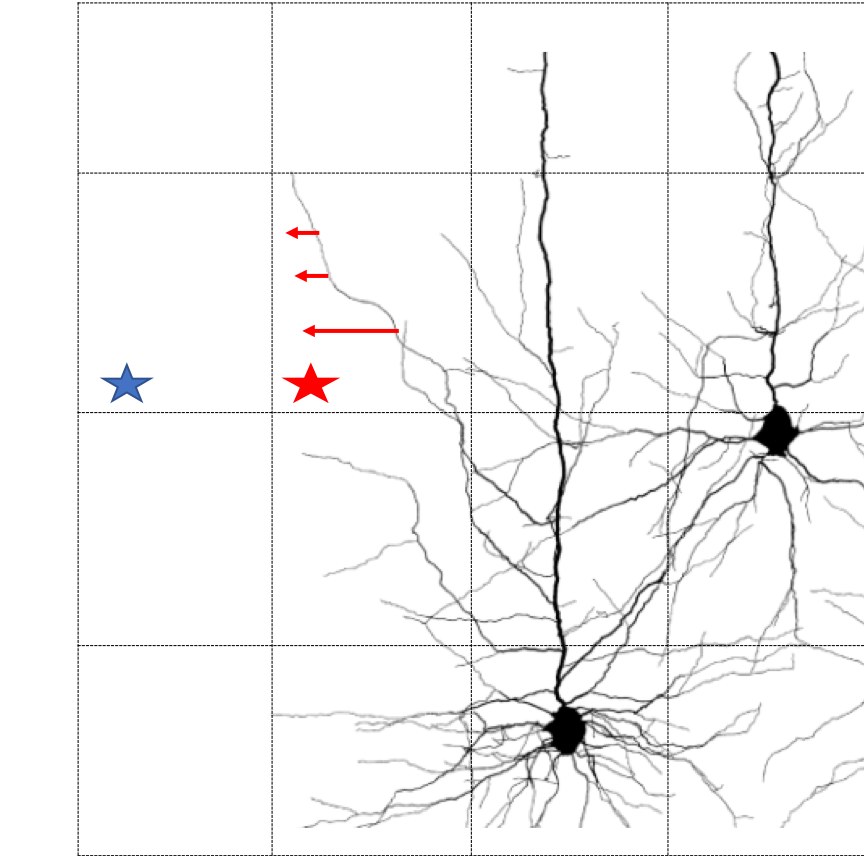
\includegraphics[width=0.5\textwidth]{Figures/Eldiff/KNP.png}
\end{center}
\caption{\textbf{KNP scheme}. Blue star: Mesh cell containing no neuronal sources, so that $C=0$. Red star: Mesh cell containing neural sources. Here $C$ can be computed by summing over all neuronal transmembrane currents, including the capacitive current, and dividing by the volume of the mesh cell. LAGE LITT MER INFORMATIV FIG HER OM VI SKAL HA FIG HER.}
\label{Eldiff:fig:KNPmesh}
\end{figure}


\subsection{Do diffusion potentials matter?}
Due to the computational challenges they impose, it is tempting to make the assumption that diffusive currents contribute so little to the extracellular potential that we don't have to bother with them. This is what normally is being done, as most theoretical studies of extracellular potentials are based on standard VC theory. For most purposes, this is probably a good approximation, but its validity depends on one of the two following criteria being met:

\begin{enumerate}
\item C1: The magnitude of diffusive currents is much smaller than the magnitude of Ohmic drift currents.
\item C2: The frequency of diffusive currents is much smaller than the frequency of the CSD and the Ohmic drift currents. 
\end{enumerate}

The first criterion is general and quite intuitive. If C1 holds, the last term in eq. \ref{eq:eldiffCSD2} becomes much smaller than the other two terms, and standard VC theory will give accurate predictions of $\phi$. As we shall see below, it is quite likely that C1 is violated under many physiological conditions. If so, the second criterion (C2) may still come to our rescue, as in most experiments, extracellular potentials are recorded using electrode systems with a lower cut-off frequency of 0.1-1 Hz \cite{Einevoll2007}. As diffusive currents are proportional to concentration gradients, which generally vary at a much slower time scale than $\phi$, diffusive contributions to $\phi$ are often direct-current (DC) like, i.e., almost constant in time. If so, they will not be picked up in recordings using standard electrode systems, only in experiments using DC electrodes. The question regarding their contribution to standard measurements is then whether they are DC-like enough. 

In the two following sub-sections we shall explore when and to which degree the criteria C1-C2 are likely to be met under physiological conditions.

\subsubsection{Magnitude of diffusion potentials.}
Here, we will make some crude estimation of the magnitude that we can expect diffusion potentials to have in neural tissue. To make these, make the following simplifications of eq. \ref{eq:eldiffCSD2}): Firstly, diffusion potentials depend solely on extracellular concentration gradients, and not on the instantaneous activity of neurons. Let us therefore assume that $CSD = 0$, and consider the extracellular dynamics is governed by
\begin{equation}
\nabla \cdot (\sigma_e\nabla\phi_d) = - \nabla \cdot \left (\sum_k{F z_k \tilde{D_k}{\bf \nabla} c_{k}} \right), 
\label{eq:eldiffCSD3}
\end{equation}
where we have denoted the potential $\phi_d$ since, in this case, it will exclusively be evoked by diffusion. Let us further consider a system with closed boundaries, so that no current can enter/leave the system. In that case, we may simply skip the first nabla, and take:
\begin{equation}
\sigma_e\nabla\phi_d = -\sum_k{F z_k \tilde{D_k}{\bf \nabla} c_{k}}, 
\label{eq:diffpot}
\end{equation}
Essentially, eq. \ref{eq:diffpot} states that the Ohmic drift current and diffusive current must cancel each others at each point in space, i.e., that if no current enters the system from the outside, no net current should be observed anywhere inside the system. The diffusion potential is thus the potential that we must have in the system for this to be the case. 

Finally, due to the linearity in eq. \ref{eq:diffpot}, the diffusion potential between two points in space is a direct function of the the ionic concentrations at these two points. Hence, it is sufficient for our task to consider a simple two-compartment system (like that in Fig. \ref{Eldiff:fig:diffpot}). For two-compartment systems, eq. \ref{eq:diffpot} further simplifies to:

\begin{equation}
\Delta \phi_d = \frac{F}{\bar{\sigma_e}} \sum_k{z_k \tilde{D}_k \Delta c_k}
\label{eq:diffpot2}
\end{equation}
where $\Delta c_k = c_{k}^{2} - c_{k}^{1}$ and $Delta \phi_d = \phi_d^{2} - \phi_d^{1}$ denote the concentration and potential difference between compartments 1 and 2. Within each compartment, $\sigma_e$ can be determined from the ionic concentrations by use of eq. \ref{eq:sigma1}. However, since we for this problem need the conductivity experienced by an Ohmic current traveling between the two compartments, we have in eq. \ref{eq:diffpot2} used the average $\sigma_e$ of the two compartments:
\begin{equation}
\sigma_e = \frac{F}{2\psi}\sum_{k} \left(\tilde{D}_k z_{k}^2 c_{k}^{1} + \tilde{D}_k z_{k}^2 c_{k}^{2} \right).
\label{eq:sigma2}
\end{equation}

Based on eq. \ref{eq:diffpot2}, we make some estimates of the magnitude of the diffusion potential for some test examples.

\begin{itemize}

\item {\bf Diffusion potential under spreading depression:} The most extreme extracellular concentration shifts in the brain occur under the pathological condition called spreading depression, where the extracellular K$^+$ concentration can change by several tens of millomolars. In an an example from hippocampus, the K$^+$ concentration was about 30 mM higher at the bottom hippocampal layer than at the top hippocampal layer (Fig. 1a in \cite{Herreras1993}). In that experiment, only K$^+$ concentrations were recorded. However, we may give a crude estimate of the diffusion potential between the top and bottom of hippocampus by making some simple assumptions of the other ion concentrations: (i) We assume that the top layer of hippocampus remained at baseline concentrations. In the experiment, this seemed to be close to the case for $c_K$ \cite{Herreras1993}. In the top layer, we may therefore assume some rather typical baseline concentrations with $c_{Na} = 150$ mM, $c_{K} = 3$ mM and $c_{Cl} = 153$ mM. (ii) In the bottom layer, we assume that the $c_K$ was 30 mM above baseline, and that the increase in $c_K$ was compensated by an identical decrease in $c_{Na}$, so that electroneutrality was preserved. A plausible mechanism behind this would be that all concentration shifts were due to neuronal AP firing, i.e., neurons exchanging Na$^+$ for K$^+$. With these assumptions, we have $c_{Na} = 120$ mM, $c_{K} = 33$ mM and $c_{Cl} = 153$ mM in the bottom layer. Plugging the top layer and bottom layer co ncentrations into eq. \ref{eq:diffpot2}, we obtain a diffusion potential $\Delta \phi_d \sim 1$ mV across the hippocampal depth.

\item {\bf Diffusion potential in cortex during neuronal hyperactivity:} In several experimental papers, extracellular concentration shifts of selected ions have been recorded during induced neuronal hyperactivity and seizure activity \cite{kriv1975, nicholson1978, Dietzel1982, somjen1986, Dietzel1989}. The main focus of these works are typically on $c_K$, which is the most critical extracellular concentration due to its low baseline value. In these experiments, $c_K$ can typically change from a baseline value around 3 mM up to a ceiling level between 8-12 mM before the dynamics becomes pathological and is driven into spreading depression. Dietzel et al. estimated the concentration shifts in both $c_{K}$, $c_{Na}$ and $c_{Cl}$, and cased on a series of recordings, they estimated that the maximal diffusion potential that could be expected under their experimental condition was 0.4 mV \cite{Dietzel1989}.

\item{\bf Diffusion potential during normal activity:} It is difficult to find experimental data that allows us to estimate diffusion potentials in the brain under "normal" conditions, and the question as to whether concentration gradients are present in a given brain region probably depends on the processing state it is in. However, recordings from anesthetized cat cortex have shown that even during the resting state, $c_K$ may exhibit small-amplitude (0.5 mM) fluctuations \cite{MCCREERY1983}. In experiments recording the response in cortex to moderate (not seizure inducing) stimuli applied in the thalamus, cortical $c_K$ increases were found to have a depth profile, and vary by about 2 mM between different cortical layers \cite{Cordingley1978}. Thus, it seems likely that there should be some concentration gradients present in neural systems, and that e.g., a concentration difference of about 1 mM between the top and bottom of cortex or hippocampus would not be unlikely under normal processing. If we repeat the calculation from spreading depression, but assume that $c_{K}$ and $c_{Na}$ in the bottom layer were increased/decreased by 1 mM instead of 30 mM, we get a diffusion potential of about $33 \mu$V. This is of the same magnitude as potentials typically recorded in LFP recordings. 

\end{itemize}

Based on the above estimates, diffusion potentials can not as a generality be expected to be so small that they can be ruled out as possible contributors to the LFP. 


\subsubsection{Frequency of diffusion potentials}
\ghnote{Krevende kapittel. Sammenligne noen powerspectra her. Regne ut et par selv, ala Gratiy.} 

Previous computational studies have predicted that effects of diffusion on extracellular potentials are not necessarily small, but tend to be very slow, meaning that they will only affect the very low-frequency components of $\phi$ \citep{Halnes2016, Halnes2017}. This is due to the diffusive current being a direct function of ion concentrations $c_k$, which on a large spatial scale typically vary on a much slower time scale (seconds-minutes) than the fluctuations in $\phi$ that we commonly are interested in (milliseconds-seconds). Furthermore, electrodes used to record $\phi$ typically have a lower cutoff frequency of 0.1-1Hz \citep{Einevoll2013}, which means that most of the tentative diffusive contribution will be filtered out from experimental recordings. It may therefore be a good approximation to neglect the diffusive term, except in the case of pathologically dramatic concentration variations.

\include{Ch6-schemes}

%\newpage
{\huge Part 2}
\section{Spikes}

\ghnote{Tekst under klippet fra bokkapittel. Tenker at vi trenger en intro her som forklarer dette.}
Extracellular potentials measured within neural tissue are often split into two separate frequency domains, which reflect different aspects of the underlying neural activity. The low frequency part, the local field potential (LFP), is thought to mostly reflect synaptic input to populations of pyramidal cells, while the high-frequency part, the multi-unit activity (MUA), reflects the population spiking activity (Fig.~\ref{XX:fig:LFP_MUA}).
%%%%%%%%%
% Figure
%%%%%%%%%
\begin{figure}[!ht]
\begin{center}
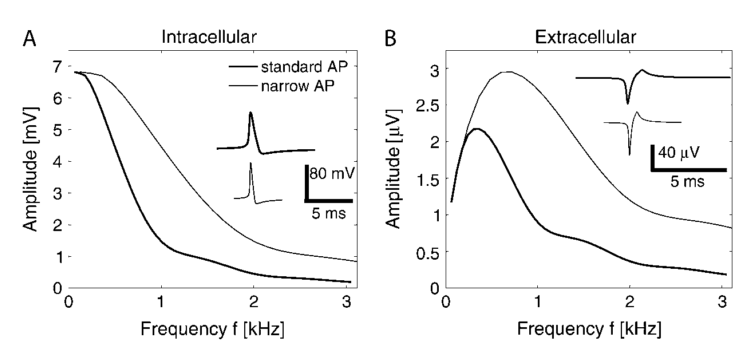
\includegraphics[width=0.6\textwidth]{Figures/Spikes/Spikes-eap_illustration.png}
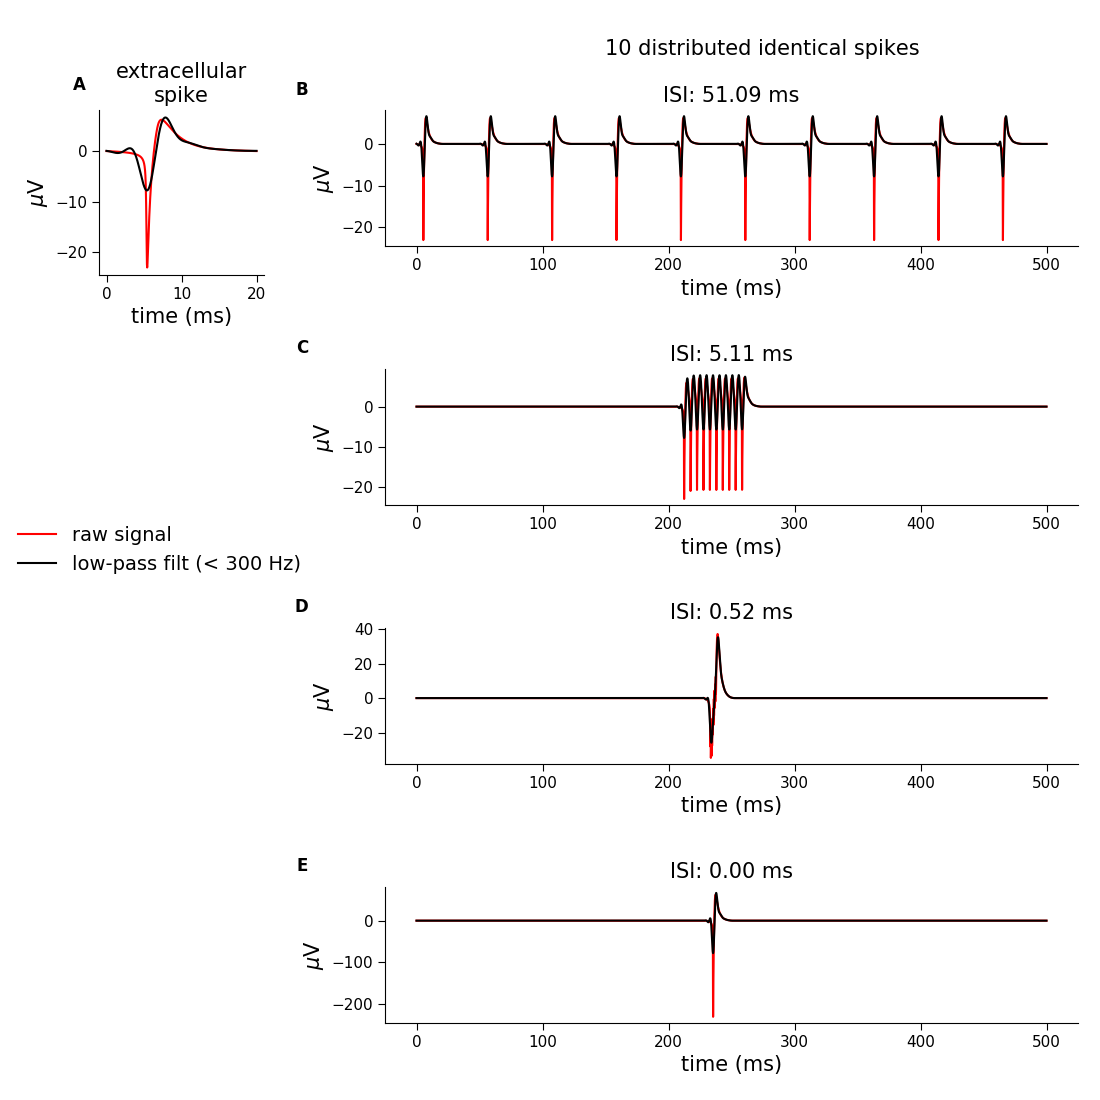
\includegraphics[width=0.6\textwidth]{Figures/Spikes/Spikes-LFP_spike_effect_test_300Hz.png}
\end{center}
\caption{\textbf{Potential EAP figures} 
Common misconception that spikes only have frequency content above a few hundred Hz. Delta pulse have flat frequency spectrum.}
\label{Spikes:fig:freq_dep}
\end{figure}

\subsection{Spikes in neurons with passive dendrites} 
\label{Spikes:sec:EP-spikes}
%Kjernereferanse: \citep{Pettersen2008a}
%
%Perhaps start this by showing membrane potentials for cells with passive dendrites. 
%Then show extracellular signatures.


%%%%%%%%%%
% Figure: Intracellular and extracellular action potentials
%%%%%%%%%%
%\begin{cnfigure}{Figures/mm/EP-spike-Henze-w100-r150}
\begin{figure}[!ht]
\begin{center}
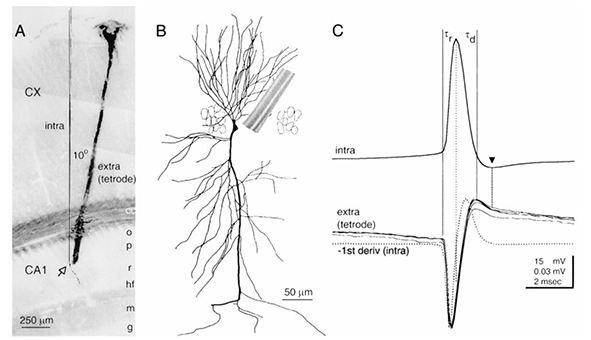
\includegraphics{Figures/Spikes/Spikes-Henze-w100-r150}
\end{center}
\caption{\textbf{Simultaneous recording of intracellular and extracellular action potentials (`spikes').}
Adapted from \citet{Henze2000}.
\gen{Figure + caption to be updated}
}
\label{Spikes:fig:Henze}
\end{figure}
%%%%%%%%%%%


%The recording of spikes, the EPs corresponding to action potentials in individual neurons, has been
%key for learning about how neurons and neural networks function in live brains. 
When a sharp electrode is placed close to the soma of a neuron, an intracellular action potential will be seen
extracellularly as a sharp `spike' in the EP (Figure~\ref{Spikes:fig:Henze}). The magnitudes of these signals are quite different. While intracellular action potentials have amplitudes of $\sim$100~mV, the amplitudes of extracellular
spikes are typically less than 1~mV. Nevertheless, the detection of these spiking events from the recorded signal is relatively easily, and faithful records of the firing activity of neurons can be obtained. Such measurements have been instrumental in learning about \index{neural representations}, that is, how neurons in different parts of the brain, for example, encode information about visual and other sensory input. 

%%%
\subsubsection{Spikes from two-compartment neuron models}
\label{Spikes:sec:EP-spikes-two-compartment}
%%%
Intracellular potentials can be modelled with a single-compartment neuron model as described in Chapter~3.
However, as described in the previous section, 
a two-compartment neuron model is the simplest model that can produce an extracellular potential such as a 
spike. An example of this is provided in Figure~\ref{Spikes:fig:TwoCompartment} where active sodium and potassium conductances are added to the  soma compartment of an otherwise passive neuron model. 
The membrane potential during a spike is illustrated in the right panel, and the  
corresponding EP is computed from Equation~\ref{Spikes:equation:Ve-two-compartment}. Around the soma a characteristic
EP spike with a sharp negative peak followed by a slower positive hump is seen, in accordance with typical experimental
spike recordings as exemplified by Figure~\ref{Spikes:fig:Henze}. Around the dendrite compartment inverted
spikes of the same sizes are seen, but such inverted spikes are rarely, if ever, seen in experiments. This suggests that
modelling dendrites as a single compartment is inadequate when one is interested in predicting the detailed spatial pattern of 
spike shapes that would be recorded by an electrode at different positions around a neuron.                                                                                                                                                                                                                                                                                                                                                                                                                                                                                                                                                                                                                                                                                                                                                                                                                                                                                                                                                                                                                                                                                                                                 

%%%%%%%%%%
% Figure: Spike from two-compartment model
%%%%%%%%%%
%\begin{cnfigure}{Figures/mm/EP-spike-TwoCompartment-w100-r150}
\begin{figure}[!ht]
\begin{center}
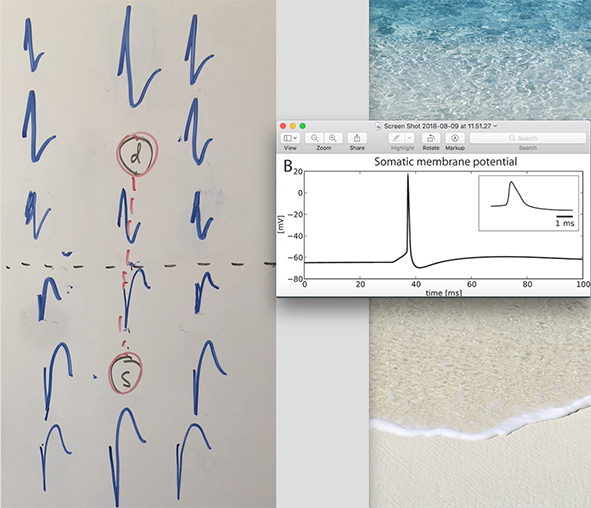
\includegraphics{Figures/Spikes/Spikes-TwoCompartment-w100-r150}
\end{center}
\caption{\textbf{EP (spike) from action potential for a two-compartment neuron model with active sodium
and potassium conductances in the soma compartment}. Computed from 
Equation~\ref{mm:equation:Ve-two-compartment}.
Left panel shows the EP at different spatial positions, while right panel shows the corresponding
soma membrane potential during the action potential. 
\gen{Figure + caption to be updated}
}
\label{Spikes:fig:TwoCompartment}
\end{figure}

%%%
\subsection{Spikes from multi-compartment neuron models}
\label{Spikes:sec:EP-spikes-multi-compartment}
%%%
A more detailed picture of spike shapes is obtained by considering a detailed multi-compartmental neuron model
with a comprehensive branching structure typical for real neurons as in Figure~\ref{Spikes:fig:MultiCompartment}.
With this dendritic morphology the membrane currents through the dendrites are spread over a larger membrane area.
As a result, Equation~\ref{Spikes:equation:Ve-multi-compartment} predicts that the largest EP spikes will be seen
around the soma for the example pyramidal neuron in Figure~\ref{Spikes:fig:MultiCompartment}.  
Around the apical dendrites, the spikes will still have an inverted shape compared to spikes close to the soma. 
However, their amplitudes will be small, only a few microvolts, so they will not be seen in most experiments.

As for the two-compartment spike model, the spike amplitude in Figure~\ref{Spikes:fig:MultiCompartment} 
decays sharply with distance from the neuron. In addition, the spike width increases
with distance as demonstrated by the insets at two example positions. For the large spike recorded next to
the soma the half-width of the spike is $\sim$0.6~ms, while at the position outside the dendrite, the half-width is increased to
$\sim$0.7~ms. This corresponds to a low-pass filtering in the sense that the distant EP has lost some 
high-frequency components compared to the EP close to the soma. This filtering effect is absent for the spike generated by the 
two-compartment neuron model, and reflects that the cable properties of dendrites are important in determining 
also the shape of recorded spikes.   

%%%%%%%%%%
% Figure: Spike from multi-compartment model
%%%%%%%%%%
%\begin{cnfigure}{Figures/mm/EP-spike-MultiCompartment-w100-r150}
\begin{figure}[!ht]
\begin{center}
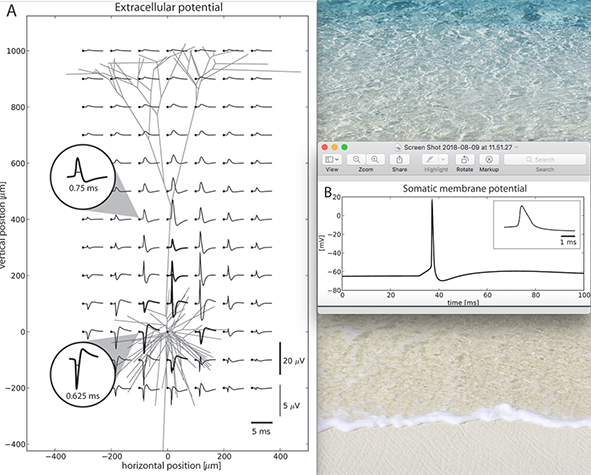
\includegraphics{Figures/Spikes/Spikes-MultiCompartment-w100-r150}
\end{center}
\caption[]{\textbf{EP (spike) from action potential for a multi-compartmental neuron model}. Active sodium
and potassium conductances in the soma compartment and computed from 
Equation~\ref{XX:equation:Ve-multi-compartment}.
Left panel shows the EP at different spatial positions, while right panel shows the corresponding
soma membrane potential during the action potential. 
\gen{Figure + caption to be updated. Change to Hay-model,}
}
\label{Spikes:fig:MultiCompartment}
%\figpermOurs
\end{figure}

%%%
\subsection{Spikes from ball-and-stick neurons}
\label{Spikes:sec:spike-widths-amplitudes}
%%%
%\todo{June 2019: Make equivalent of old Figs. 12.6 for ball and stick?}
%%
The extracellular measurement of spikes from a neuron in living brains is blind in the sense that it is
unknown what type of neuron is recorded from when an electrode is lowered into the brain.
Some neuron types produce spikes with larger amplitudes and/or broader shapes than
others, and as seen in Figure~\ref{Spikes:fig:MultiCompartment} both the shape and amplitude 
depend critically on recording positions. Large spike amplitudes imply that they will be more dominant in electrical recordings,
and this bias should ideally be considered in the analysis of joint recordings 
of spikes from many neurons.

%%%%%%%
%% FIGURE - ball-and-stick spike
%%%%%%%
%\begin{figure}[t]
%  \multifigurebox{}{}{%
%    \vbox{%
%      \hspace*{8mm}\includegraphics{Figures/network/extracellular-arrangement}\\
%      \includegraphics{Figures/network/extracellular}}}
%  \caption{\emph{Simulation of \term{extracellular field potential}s. Extracellular
%    electrodes (black, grey, blue and dark-blue) are placed
%    close to a ball-and-stick model neuron with an active soma and
%    synapses on its dendrite. The soma is 40\uum long and 40\uum
%    in diameter. The single dendritic cable is 200\uum long and 4\uum in
%    diameter. The top traces show intracellular recordings when the
%    synapses are activated enough to cause an action potential to be
%    fired.  Traces are from the soma (black), halfway down the
%    dendrite (blue) and in the distal dendrite (dark-blue).
%    The initial synaptic stimulation can be seen in the dendritic
%    traces. The lower traces show the extracellular recordings
%    corresponding to the electrodes of the same colour.  During the
%    synaptic stimulation, the dendrites act as a sink of extracellular
%    current and the soma acts as a source. This can be seen in the
%    negative deflection of the extracellular potential in medial and
%    distal dendrites and the positive deflection of the extracellular
%    potential close to the soma. During the action potential, the soma
%    is a sink of current and the dendrites are current sources; this
%    is reflected in the large negative deflection of the extracellular
%    potential close to the soma and the smaller deflections of the
%    extracellular potential near the dendrites. As the neuron
%    repolarises, the roles of the soma and dendrites are again
%    reversed.} 
%        \gen{Revise: Figure and caption copied directly from first edition. Must be adapted.}}
%  %\figpermOurs
%  \label{mm:fig:extracellular}
%\end{figure}
%%%%%%%%%%%%%

 
To understand the link between the morphology of neurons and spikes amplitudes and shapes
it is convenient to consider ball-and-stick neurons where a dendrite cable `stick' is connected to a point-like soma.
%The relation between the intracellular action potential and the corresponding extracellular spike for such a 
%neuron is illustrated in the example in Figure~\ref{mm:fig:extracellular}.
Despite its simplicity, the ball-and-stick neuron model exhibits the key qualitative features observed in
Figure~\ref{Spikes:fig:MultiCompartment} 
when the multi-compartmental EP formula in  Equation~\ref{XX:equation:Ve-multi-compartment}
is used; that is, rapid attenuation of spike amplitude 
and increased spike width as the distance from the soma increases.
Figure~\ref{Spikes:fig:ball-and-stick-results}
shows the distance dependence of these spike measures both for a detailed multi-compartmental pyramidal neuron model 
and ball-and-stick neurons (Figure~\ref{Spikes:fig:ball-and-stick-neuron-models}).
While the spike width and amplitude of the multi-compartmental neuron are larger than for
the two example ball-and-stick neurons (with short and long dendrite sticks, respectively), 
the shapes of the curves are similar. Note also that the results for a ball-and-stick neuron with an infinitely long dendritic stick is
effectively identical to the long-stick results in the figure~\citep{Pettersen2008}.
\gen{From David Sterratt: The frequency dependence here comes from intracellular properties? If so, would be great to make it clear.}


%%%%%%%%%%
% Figure: Neuron models considered in plot of spike widths and amplitudes
%%%%%%%%%% 
%\begin{cnfigure}{Figures/mm/EP-spike-ball-and-stick-neuron-models-w43-r300}
\begin{figure}[!ht]
\begin{center}
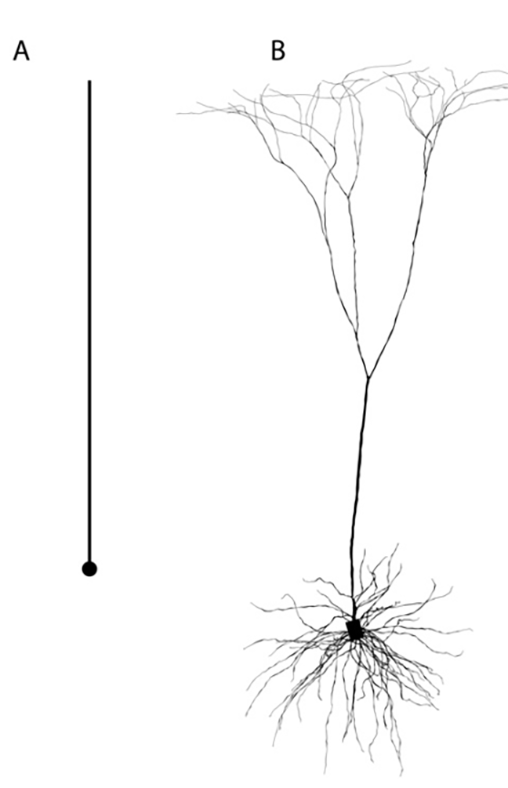
\includegraphics{Figures/Spikes/Spikes-ball-and-stick-neuron-models-w43-r300}
\end{center}
\caption[]{\textbf{Neuron models considered in results in Figure~\ref{Spikes:fig:ball-and-stick-results}}. 
\gen{Figure + caption to be updated.}
Adapted from \citet{Pettersen2008}.
}
\label{Spikes:fig:ball-and-stick-neuron-models}
%\figpermOurs
\end{figure}

To understand the physical origin of these results it is easier to consider each frequency 
component of the action potential separately. From Fourier theory it follows that any signal
can be written of waves with different frequencies, so-called Fourier components (see sidebox).  
This is illustrated in Figure~\ref{Spikes:fig:ball-and-stick-frequency} where the weight of the different frequency components needed to
represent the intracellular action potential (membrane potential) and extracellular spike, respectively, are shown.
A key observation here is that for the extracellular spike, the largest
contributions comes from frequencies larger than 100~hertz.
%\todo{DCS: Ensure Figures/mm/dipole-comparison-w43-r300.png is committed
%  to git repository and then uncomment above line.}

For the ball-and-stick neuron, a membrane current entering the soma has to return to ECS through the cable
stick, see Figure~\ref{Spikes:fig:ball-and-stick-sketch}.
When an oscillating membrane current is entered through the soma, the spatial pattern of return current will depend on the frequency of the oscillation due to the capacitive properties of the membrane: For higher frequencies the capacitive membrane current will be larger, and the 
membrane effectively more leaky. Thus the injected soma current will return closer to the soma for higher frequencies, 
as  seen in the inset in Figure~\ref{Spikes:fig:ball-and-stick-sketch}.  


%%%%%%%%%%
% Figure: Action potential and its frequency content
%%%%%%%%%%
%\begin{cnfigure}{Figures/mm/EP-spike-ball-and-stick-frequency-w90-r150}
\begin{figure}[!ht]
\begin{center}
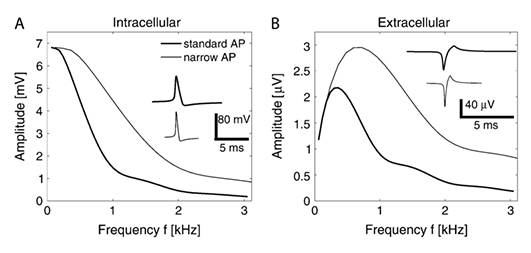
\includegraphics{Figures/Spikes/Spikes-ball-and-stick-frequency-w90-r150}
\end{center}
\caption[]{(a) Action potential used in simulations in Figure~\ref{Spikes:fig:ball-and-stick-results}(inset) 
and its frequency content.
%The intracellular spike width is defined as the
%width of the AP at half amplitude and is 0.55~ms for the standard
%AP, and half the value for the narrow AP. 
(b) Frequency content of example extracellular spike.
Inset: Typical spike shape computed a distance $r=10~\mu$m
perpendicular to the dendrite at the level of soma for a ball-and-stick 
neuron with diameter $d=2~\mu$m and infinite dendrite length.
Here the intracellular action potential in left panel was imposed as a voltage-clamp in the soma.
The extracellular spike width is defined as the width of the negative phase at 25\% of its maximum
amplitude and is 0.44~ms for the example spike.
The amplitude (peak-to-peak value) of the spike is $56~\mu$V  
\gen{Figure + caption to be updated. Will only include standard AP in final figure.} 
Adapted from \citet{Pettersen2008}.}
\label{Spikes:fig:ball-and-stick-frequency}
%\figpermOurs
\end{figure}

To compute the EP generated by an imposed oscillatory current, the stick must be divided into small compartments  
and the multi-compartmental EP formula in Equation~\ref{XX:equation:Ve-multi-compartment} used. 
This in general requires detailed knowledge of the resulting membrane currents in all compartments. 
While these can be computed for the ball-and-stick neuron (see, for example, \citet{Pettersen2014}), 
the resulting formula for the EP becomes cumbersome and difficult to interpret. 
However, as shown in XX
%Box~\ref{mm:box:ball-and-stick-spikes} 
some useful insights can be obtained in two limiting cases: the recording being very near to the soma or very far from the soma.

For recording positions very close to the soma, the contribution from the soma current will dominate 
in the sum in Equation~\ref{XX:equation:Ve-multi-compartment}. In this case the distance from the electrode
to the return currents in the dendrite will be much larger than the distance to soma. With only the contribution from
the soma compartment included, the amplitude $|\hat{V}_\mathrm{e,near}(f,\vec{r})|$  
of the EP signal for each Fourier component with frequency $f$ is found to be
%
\begin{equation}
  |\hat{V}_\mathrm{e,near}(f,\vec{r})| 
  \propto \frac{d^{3/2}}{r} \sqrt{ \frac{f C_\mathrm{m}}{R_\mathrm{a}} }  |\hat{V}_\mathrm{s}(f)| 
  \label{Spikes:equation:Ve_near}
\end{equation}
%
The suffix `near' is added because this expression only applies in the `near-field' limit, that is,
close to the soma.
$|\hat{V}_\mathrm{s}(f)|$ is the amplitude of Fourier component of the soma membrane potential at the same
frequency (see Figure~\ref{Spikes:fig:ball-and-stick-frequency}). Further, $d$ is the diameter of the dendritic
stick, $C_\mathrm{m}$ is the specific membrane capacitance, and $R_\mathrm{a}$ is the specific axial resistance.  
One of the predictions from the formula in Equation~\ref{Spikes:equation:Ve_near} is that the amplitude of each Fourier component decays
as $1/r$ when moving away from soma (yet staying within distances where the `near-field' approximation is still applicable).
Since this applies to all Fourier components which together constitute the action potential, this implies that the amplitude of the 
spike will decay as $1/r$ in this regime as well.
\gen{From David Sterratt: Intuition for the relationship witd $d, C_m, f, r_a$.}

For recording positions far away from the soma, the contribution from return membrane currents must be taken into
account in the sum in Equation~\ref{mm:equation:Ve-multi-compartment}. An approximate way of doing this is to
assume all return currents to leave the dendrite at a single point on the dendrite. Then we have 
a current dipole where the transmembrane current entering at the soma is balanced with a oppositely directed current
with the same magnitude leaving at a single point on the dendrite. The current dipole length is then given by the distance
between the soma and the dendritic position of the return current. An estimate of this length is provided by the 
frequency-dependent length constant  $\lambda_\mathrm{AC}(f)$  corresponding to the weighted mean of the positions of the return currents along
the dendrite stick (see Box~\ref{mm:box:ball-and-stick-spikes}). 
Then with the use of expression for the EP around a current dipole in 
Equation~\ref{mm:equation:Ve-dipole-p}:
%%%
\begin{equation}
  |\hat{V}_\mathrm{e,far}(f,\vec{r})|  \propto d^{2} \frac{|\cos \theta| }{r^2  R_\mathrm{a}}  |\hat{V}_\mathrm{s}(f)| 
  \label{mm:equation:Ve_far}
\end{equation}
%%%
The suffix `far' is addeds because this expression only applies in the `far-field' limit, that is,
far away from the soma. A first observation from this formula is that the EP is no longer radially symmetric, and depends both on the radial distance $r$ from the neuron and  the angle $\theta$ with the dipole axis, that is, the direction of the dendritic stick  (see Box~\ref{mm:box:dipolar-EP}). The amplitude will be largest
above and below the neuron where $\theta=0^\circ$ and $\theta=180^\circ$, respectively. In the sideways direction 
($\theta \sim 90^\circ$) the EP will be much smaller, as is characteristic for spatial pattern of potentials around a current
dipole as illustrated in Figure~\ref{mm:fig:EP-spike-TwoCompartment}. A qualitatively similar dipolar pattern, although not so distinct,
is also seen for the spike generated by the biophysically detailed multi-compartment neuron in Figure~\ref{mm:fig:EP-spike-MultiCompartment}.

Another difference of this far-field expression with the near-field expression in Equation~\ref{mm:equation:Ve_near}, is that the
amplitude decays as $1/r^2$, characteristic for potentials around dipolar sources, rather than $1/r$ which is characteristic for potentials around 
a single source. This transition from a $1/r$ `monopolar' regime to a $1/r^2$ dipolar regime is indeed observed in
the spike-amplitude panel in Figure~\ref{mm:fig:EP-spike-ball-and-stick-results}.

There are several qualitative insights regarding the sizes and widths of spikes that can 
be found from the near-field and far-field formulae in Equations~\ref{mm:equation:Ve_near} and 
\ref{mm:equation:Ve_far}, respectively. One relates directly to the shape of the spike:
in the near-field expression, the high-frequency components of the spike is amplified 
compared to the low-frequency components, that is, $\hat{V}_\mathrm{e,near}(f,r) \propto \sqrt{f}$.
Thus close to the soma the spike is observed to be sharper than the intracellular action potential
as observed in the insets in Figure~\ref{mm:fig:EP-spike-ball-and-stick-frequency}. 
In the far-field regime there is no such high-frequency amplification ($\hat{V}_\mathrm{e,near}(f,r) \propto f^0 \sim 1$).
As a consequence, spikes measured far away from the soma will have less high-frequency content than those measured close to soma.
Thus the far-away spikes will be blunter and have larger spike widths as seen in the spike-width panel of 
Figure~\ref{mm:fig:EP-spike-ball-and-stick-results}.

The spike amplitude is proportional to $d^{2}$ far away from the soma and $d^{3/2}$ close to the soma,
where $d$ is the diameter of the dendritic stick diameter.
This implies that far-way from the soma the spike amplitude is proportional to the cross-sectional area of the dendrite.
Close to the soma, the spike amplitude also increases with dendrite diameter, but not so prominently as far away.
Another observation is that the spike amplitude is independent of the membrane resistance $R_\mathrm{m}$ of the dendrite; only the membrane 
capacitance $C_\mathrm{m}$ and the axial resistance $R_\mathrm{a}$ matter, 
This reflects that the frequencies dominating the spike are so high that the capacitive membrane current 
(governed by $C_\mathrm{m}$) is much larger than the ionic membrane current  (governed by $R_\mathrm{m}$). 
%\todo{DCS: I'm wondering if we need more details on frequency-dependent cable theory, beyond Eq. 5.11.}

An overall observation is that the spike is quite local, that is, the amplitude of the spike decays rapidly with distance from the neuron soma. For the pyramidal neuron considered in 
Figure~\ref{mm:fig:EP-spike-ball-and-stick-results}, for example, the spike amplitude decays from being about
300 microvolts a distance 20 micrometers from the soma center to being only about 10 microvolts a
distance 100 micrometers away. This rapid decay eases the interpretation of recorded spikes, since it implies
that in practice an electrode contact will only pick up spikes from neurons with somas positioned within a radius of some tens of micrometers.


%%%%%%%%%%
% Sidebox: Fourier sum
%%%%%%%%%%
%\begin{sidebox}
\subsubsection{\gex{Side box: Fourier sum}}
\gen{This subsection used to be a side box in the Sterratt chapter}.
Time signals, such as the time course of a spike $V_\mathrm{e}(t)$,  can conveniently 
be represented as a sum of \index{Fourier components} with different frequencies $f$. 
Such a Fourier sum can be constructed in
various ways. The derivations in 
Section~\ref{Spikes:sec:spike-widths-amplitudes}, building on \citet{Pettersen2008}, use the  
convention that a time signal $S(t)$ is the real part of the complex sum $\sum_{f}  \hat{S}(f) \exp (j 2 \pi f t)$. 
Here $j$ is the unit of imaginary numbers, and  $\hat{S}(f)$ is in general a complex number. 
%\end{sidebox}
%

%%%%%%%%%%
% Figure: Spike widths and amplitudes
%%%%%%%%%%
%\begin{cnfigure}{Figures/mm/EP-spike-ball-and-stick-results-w100-r150}
\begin{figure}[!ht]
\begin{center}
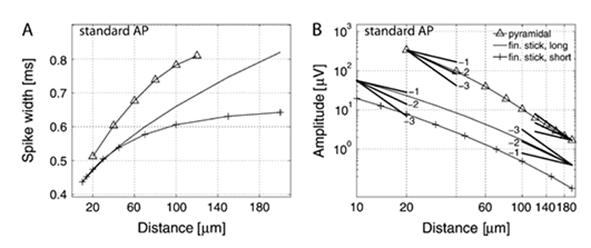
\includegraphics{Figures/Spikes/Spikes-ball-and-stick-results-w100-r150}
\end{center}
\caption[]{
Spike widths (left) and (peak-to-peak) spike amplitudes (right) as a function of
distance from soma for a detailed pyramidal cell model (pyramidal) and two
types of ball-and-stick models: long, finite ball-and-stick
model (fin.~stick, long) with diameter $d=2~\mu$m and length
$l=1$~mm and a short, finite ball-and-stick model (fin.~stick, short) with diameter $d=1~\mu$m and length $l=0.2$~mm,
see Figure~\ref{Spikes:fig:ball-and-stick-neuron-models}.
The intracellular action potential shown in the inset in the left panel of 
Figure~\ref{Spikes:fig:ball-and-stick-frequency} was imposed as a voltage-clamp in the soma.
The EP was recorded in the
somatic plane normal to the stick/primary apical dendrite. 
In right panels guidelines illustrating the power-law decays $1/r$ and
$1/r^{2}$ have been added. 
For further details see \citet[Figure 6]{Pettersen2008}.
\gen{Figure + caption to be updated.} 
Adapted from \citet{Pettersen2008}.
}
\label{Spikes:fig:ball-and-stick-results}
%\figpermOurs
\end{figure}

%%%%%%%%%%
% Figure: Frequency-dependent distribution of return currents
%%%%%%%%%%
%\begin{cnfigure}{Figures/mm/EP-spike-ball-and-stick-sketch-w70-r300}
\begin{figure}[!ht]
\begin{center}
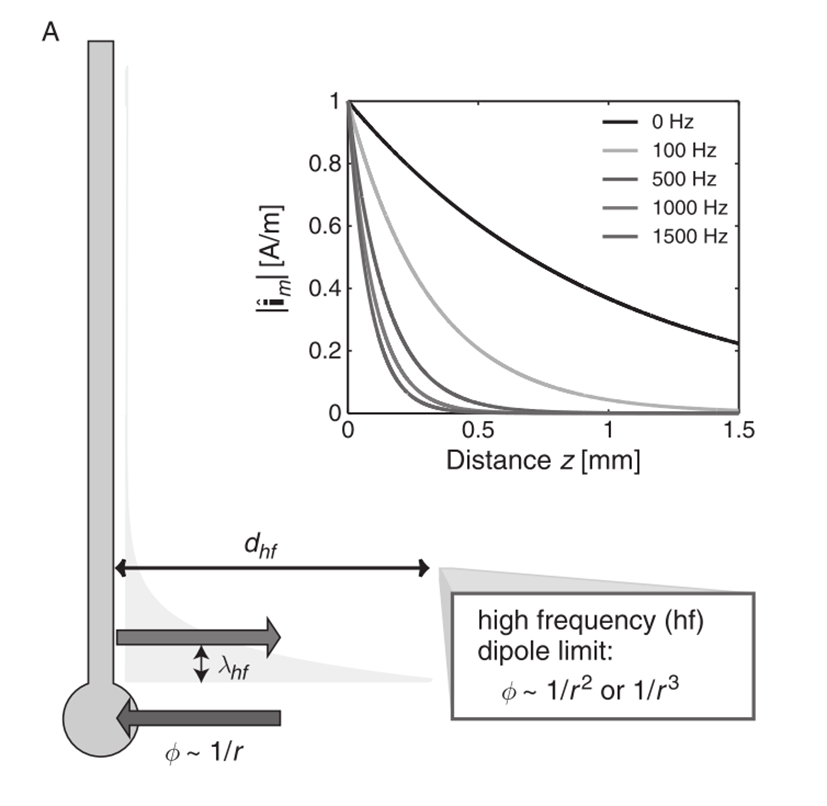
\includegraphics{Figures/Spikes/Spikes-ball-and-stick-sketch-w70-r300}
\end{center}
\caption[]{Illustration of ball-and-stick neuron and its frequency-dependent 
distribution of dendritic return currents following injection of a sinusoidal current into the soma.
The net current entering the soma will enter the dendrite as an axial current, and return to the 
ECS via the dendrite membrane. The inset shows the spatial distribution of this return current
for different frequencies. The higher the frequency, the closer the return currents will be and
the smaller the frequency-dependent length constant $\hat{\lambda}(f)$, reflecting the weighted mean 
of the return-current positions (see sidebox), will be. 
\gen{Figure + caption to be updated.} Adapted from \citet{Pettersen2012}.
}
\label{Spikes:fig:ball-and-stick-sketch}
%\figpermOurs
\end{figure}
%

%%%%%%%%%%
% Box: Ball-and-stick model for spikes
%%%%%%%%%%
%\begin{boxfloat}{Ball-and-stick model for spikes}
%  \label{mm:box:ball-and-stick-spikes}  
\subsubsection{Box: Ball-and-stick model for spikes}
\gen{This was a box in the Sterratt chapter}
To understand the dependence of spike shapes and amplitudes on model parameters for the ball-and-stick neuron, it is useful
to consider the EP set up by each of the frequency (Fourier) components of the action potentials separately. 
For recording positions $\vec{r}$ very close to the soma, the contribution from the soma current will dominate over the contributions from the dendrite 
in the sum giving the EP in Equation~\ref{XX:equation:Ve-multi-compartment}. Then the amplitude of the
predicted oscillating EP $|\hat{V}_\mathrm{e,near}(f,\vec{r})|$ is approximately given by 
%
\begin{equation}
  |\hat{V}_\mathrm{e,near}(f,\vec{r})| = \frac{|\hat{I}_\mathrm{s}(f)|}{4 \pi \sigma r} 
  \label{Spikes:box:equation:Ve_near_1}
\end{equation}
%
where $|\hat{I}_\mathrm{s}(f)|$ is the amplitude of the oscillating current through the soma membrane.
%and also the axial current entering the dendrite from the soma compartment. 
For the relatively high frequencies of most relevance for the spike, this soma current is related to the soma membrane potential 
$\hat{V}_\mathrm{s}(f)$ through~\citep{Pettersen2008}
%
\begin{equation}
  |\hat{I}_\mathrm{s}(f)| =  \frac{\pi^{3/2} d^{3/2}}{\sqrt{2}} \sqrt{ \frac{f C_\mathrm{m}}{R_\mathrm{a}} }  |\hat{V}_\mathrm{s}(f)|
  \label{Spikes:box:equation:Isoma}
\end{equation}
%
and the spike EP is thus found to be
%
\begin{equation}
  |\hat{V}_\mathrm{e,near}(f,\vec{r})| 
  = \frac{\sqrt{\pi}}{4 \sqrt{2} \sigma}
     \frac{d^{3/2}}{r} 
     \sqrt{ \frac{f C_\mathrm{m}}{R_\mathrm{a}} }  |\hat{V}_\mathrm{s}(f)| 
  \propto \frac{d^{3/2}}{r} \sqrt{ \frac{f C_\mathrm{m}}{R_\mathrm{a}} }  |\hat{V}_\mathrm{s}(f)| 
  \label{Spikes:box:equation:Ve_near_2}
\end{equation}
%
%
For recording positions further away from the soma, the contribution from return membrane currents must be taken into
account in the sum in Equation~\ref{mm:equation:Ve-multi-compartment}. An approximate way of doing this is to
assume all return currents to leave the dendrite at a single height $\lambda_\mathrm{AC}(f)$ above the soma, where 
this frequency-dependent length constant corresponds to the weighted mean of the positions of the return currents along
the dendrite stick. (The subscript `AC' denotes `alternating current'.)
Then the EP can be approximated by using the 
dipolar expression in Equation~\ref{mm:equation:Ve-dipole-p}, that is,
%%%
\begin{equation}
  |\hat{V}_\mathrm{e,far}(f,\vec{r})| =  \frac{|p(f) \cos \theta|}{4 \pi \sigma r^2} 
                                            = \frac{| \hat{I}_{s}(f) \lambda_\mathrm{AC}(f) \cos \theta|}{4 \pi \sigma r^2}   
                                                                                        \label{Spikes:box:equation:Ve_far_1}
\end{equation}
%%%
One way to define an AC length constant is as the mean value of the 
envelope of the sinusoidally varying (normalized) membrane current
$\hat{i}_\mathrm{m}$ weighted with distance $z$ from soma, 
see Figure~\ref{mm:fig:EP-spike-ball-and-stick-sketch}. 
For an infinite dendrite stick this corresponds to
%
\begin{equation}
  \lambda_\mathrm{AC}^\infty(f) = \frac{\int_0^\infty z |\hat{i}_\mathrm{m}| dz}{\int_0^\infty |\hat{i}_\mathrm{m}| dz} 
\nonumber
%=  \frac{\sqrt{2}\lambda}{\sqrt{\sqrt{W^2+1}+1}}.
\end{equation}
%

For high frequencies ($f \gg 1/2 \pi R_\mathrm{m} C_\mathrm{m}$) this is after some algebra 
found to give (see \citet[Appendix C]{Pettersen2008} for details)
%
\begin{equation}
 \lambda_\mathrm{AC}^\infty(f) =  \frac{\lambda}{\sqrt{\pi f \tau}} = 
  \frac{1}{2\sqrt{\pi}} \sqrt{\frac{d}{f R_\mathrm{m} C_\mathrm{m}}}
\label{Spikes:box:equation:approx_lambda_ac}
\end{equation}
%
where $\lambda$ is the cable length constant from 
%Chapter~\ref{XX:chap:XX}
Chapter~XX. 

%
Thus for EPs measured far away from the soma we find 
%  
\begin{equation}
  |\hat{V}_\mathrm{e,far}(f,\vec{r})|  = \frac{1}{8 \sqrt{2} \sigma} d^{2} \frac{1}{r^2  R_\mathrm{a}} 
      |\hat{V}_\mathrm{s}(f) \cos \theta | 
  \propto d^{2} \frac{|\cos \theta|}{r^2  R_\mathrm{a}} |\hat{V}_\mathrm{s}(f)| 
  \label{Spikes:box:equation:Ve_far_2}
\end{equation}
%
Equations~(\ref{mm:box:equation:Ve_near_2}) and (\ref{mm:box:equation:Ve_far_2}) describe how each frequency component of 
the soma membrane potential  $\hat{V}_\mathrm{s}(f)$ is `translated' into frequency components of the 
EP spike ($\hat{V}_\mathrm{e,near}(f,\vec{r})$ and $\hat{V}_\mathrm{e,far}(f,\vec{r})$, respectively). 
%\end{boxfloat}
%%%%%%%%%%%%%%%%%%%%%%%%%%%%%%%%%%%%%%%%%



%%%%%%%%%%
% Box: Spike sorting
%%%%%%%%%%
%\begin{boxfloat}{Spike sorting}
%  \label{mm:box:spike-sorting}
\subsubsection{\gex{Box: Spike-sorting}}
\gen{This was a Box in the Sterratt chapter}
%
\centerline{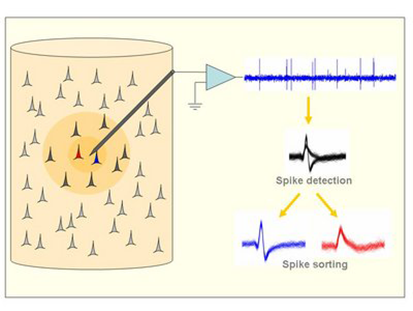
\includegraphics{Figures/Spikes/Spikes-sorting-w35-r300}}\vspace*{6pt}
%
A sharp electrode placed in brain tissue will pick up spiking signals from several neurons. 
However, the shapes of the spikes will be different for the different neurons, and this can be used to sort the spikes according to their neurons of origin. This is referred to as \index{spike sorting}, 
and is a problem of great practical importance both for neuroscience research and development of neuroprosthetic devices. 

In the present day with electrodes with hundreds or thousands of electrode recording contacts, fast and accurate automatic spike-sporting methods are needed to replace time-consuming manual spike-sorting methods~\citep{Quiroga2007}. To develop and test such automatic methods, one needs
benchmarking spiking data where the `ground truth', that is, the actual spiking times for the contributing neurons, is known~\citep{Einevoll2012}.
One use of the EP modelling scheme for spikes has been to generate such benchmarking data~\citep{CamunasMesa2013,Hagen2015,MondragonGonzalez2017}. 

Modern electrodes have numerous recording contacts, often placed only some micrometers apart. Thus a spike can be measured at several contacts
simultaneously, each contact recording a slightly different shape reflecting the different positions of the contacts relative to the spiking neuron. 
This not only allows for accurate spike sorting, but also for estimation of the spatial position of the neuron. Likewise, the spatial variation of the 
spike shape around the neuronal soma (see Figure~\ref{Spikes:fig:MultiCompartment}) 
depends on the details of the intracellular action potential and dendritic morphology thus also allowing for the 
identification of neuron type~\citep{Buccino2018}.    
\gen{Figure to be adapted from Quiroga (2007).}
%\end{boxfloat}
%%%


%%%%%%%%%%%%%%%%%%%%%%%%%%
% Box: Spike i MEA
%%%%%%%%%%    
\subsubsection{\gex{Box:Spikes in microelectrode arrays (MEAs)}}
\gen{This was a box in Sterratt book chapter}
%\begin{boxfloat}{Spikes in microelectrode arrays (MEAs)}
%  \label{mm:box:spike-MEA}
As an alternative to measuring spikes in living brains, small slices of brain tissue can be put in suitably arranged dishes
where electrophysiological cellular properties can be studied for a few hours. Such \index{\emph{in vitro}} recordings
allows for more detailed and better controlled investigations than what can be achieved in living brains. In one type of such recordings
the brain tissue is placed on a \index{micro-electrode array (MEA)}. Here the bottom of the device contains a grid of electrode
contacts picking up electrical potentials generated by the neural activity of the slice of  brain tissue placed on top of it. 
The slice and the MEA are further covered with a liquid, typically saline, to keep the cells in the brain tissue functioning for the duration
of the experiment,  see figure:
%
\begin{center}
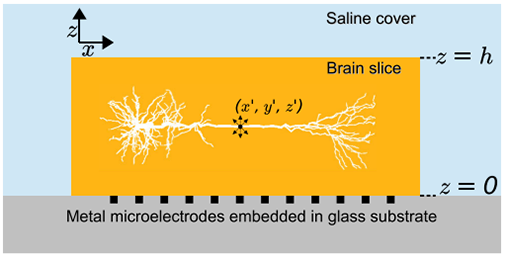
\includegraphics{Figures/Spikes/Spikes-MEA-1-w43-r300}
\end{center}
\vspace*{6pt}
%
In such measurements, the experimental set-up itself has an effect on recorded spikes. The microelectrode contacts are 
embedded in an insulating glass plate with very low electrical conductivity, while the saline has
a higher electrical conductivity than the brain slice it covers. 
For such planar step-wise discontinuities in the conductivity (assuming for the moment the MEA substrate, slice and saline
all are infinite planes) formulae analogous to Equation~\ref{XX:equation:Vr} can be derived by use of the
\index{method of images} from electrostatics, see Box~\ref{XX:box:MOI}.

While the largest effect on the recorded spike shape comes from the insulating 
glass substrate which roughly doubles the size of the recorded spikes, the figure below illustrates the 
effect from the saline covering the brain slice. As seen in the example results, the highly-conductive 
saline cover reduces the size of the recorded spike compared to the hypothetical 
situation where the saline had the same value of the electrical conductivity as the brain slice.
Figure is adapted from \citet{ness2015}.
%
\begin{center}
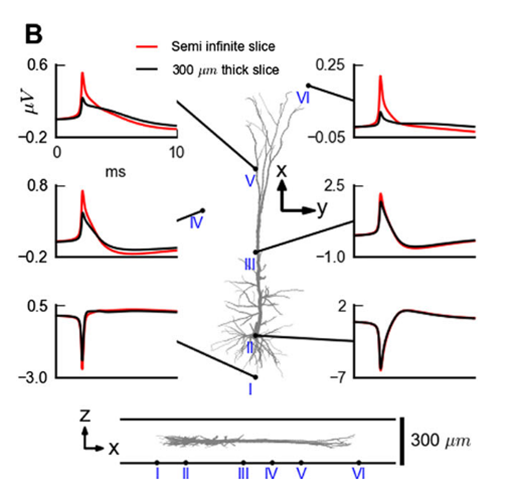
\includegraphics{Figures/Spikes/Spikes-MEA-2-w43-r300}
\end{center}
%
%\todo{DW: Too small.}
%\end{boxfloat}
%%%%%%%%%%%%%%%%%%%%%%%%%%%%%%%


While the formulae above were derived for a neuron model with a single passive dendritic stick, similar expressions can be derived for 
more complicated neuron models where several passive sticks protrude from the soma, see \citet{Pettersen2008}.
The main conclusions above hold also for these neuron models, in particular that spike widths always increase with distance and that
the amplitude of a spike is proportional to $d^{k}$ where $k\sim1.5-2$. For neurons with many dendrites attached to the 
soma, the contributions to the spike amplitude roughly adds up. A simple rule of thumb is that a neuron's spike amplitude is 
roughly proportional to the sum of the cross-sectional areas for all dendrite branches attached directly onto to the soma. Neurons with many thick
dendritic branches attached to the soma will thus generate the largest spikes. See~\citet{Pettersen2008} for further discussion.


\subsection{Spikes in neurons with active dendrites} 
Kjernereferanse: \citep{Gold2006}
Perhaps start this by showing membrane potentials for cells with active dendrites. 
Then show extracellular signatures.

\subsection{Multi-unit activity (MUA)} 
Kjernereferanse: \citep{Pettersen2008}

\subsection{Insights from MUA studies} 
\ghnote{I added this kind of subsection to most of the Part 2 - sections. I thought it might be an idea to finish the MUA, LFP, ECoG and EEG sections with summaries of what these modalities typically tell us, i.e. in terms of (i) what aspects of neural activity they reflect (spikes, synaptic inputs, dendritic ion channels, which ion channels, which kind of neurons, something on network structure, cell orientation, cortical folding etc.), and what what they can tell us about cognitive states (attentive, drowsy etc.). I am not sure about this idea, though. Maybe it will be too challenging to get an overview over the literature - we dont want to put the entire Nunez-book into the EEG-chapter.}

\section{Local Field Potentials}
\ghnote{Torbjorn will write this chapter}

\subsection{Single-neuron LFPs}
\begin{itemize}
\item Passive dendrites \citep{Linden2010}
\item Active dendrites \citep{Ness2016}
\end{itemize}

\subsection{Population LFPs}
\begin{itemize}
\item Passive dendrites 
\begin{itemize}
\item Full simulations \citep{Linden2011,Leski2013}
\item Analytical results~\citep{Einevoll2013a}
\item "Magic" simple formula \citep{Mazzoni2015}
\end{itemize}
\item Active dendrites \citep{Ness2018}
\item Kernel trick? 
\end{itemize}

\subsection{Network LFPs}
\begin{itemize}
\item Cortical LFPs from single corticothalamic neuron \citep{Hagen2017}
\item Cortical networks with passive dendrites with hybrid trick \citep{Hagen2016}
\item Cortical network with active dendrites \citep{Reimann2013}
\end{itemize}

\subsection{Insights from LFP studies} 

\section{ECoG}
\label{sec:ECoG}
\ghnote{Torbjorn or Solveig will write this chapter?}

\subsection{Insights from ECoG studies} 

\section{EEG}
\label{sec:EEG}
\ghnote{Solveig will write this chapter?}



\subsection{4-sphere model} 
Kjernereferanse: \citep{Naess2017} and Naess et al (in preparation).


\subsection{Insights from EEG studies} 

\section{MEG}
\label{sec:MEG}

\index{MEG}
\ghnote{
Here we must understand the relationship between "impressed currents" and "primary currents" as they are used in the MEG litterature, i.e., in the book Brain Signals.

So far, we have MEG only as an application-chapter. Should we have a theory chapter magnetic fields it in Part 1, or will we sneak the theory in here as we go along?}

\subsection{Insights from MEG studies} 
The human being is essentially just a very weak electromagnet. 
\section{Electrical stimulation}
\ghnote{Maybe just illustrate the fundamental principles? Who writes this? }


\section{Technology} 
\label{sec:Tech}
\ghnote{Klas will write this chapter. It will be dedicated to Elon Musk.}

\appendix
\section{Derivation of four-sphere model}
\tvnnote{Paste from LFPy 2.0 paper?}
%\tvnnote{Solveigs utledning av når strømdipol-approksimasjonen er gyldig?}
\chapter{Derivation of the current dipole approximation}
\label{app:dipoleappendix}
\tvnnote{Hmm, litt dumt at ligninger, underseksjoner og figurer alle faar navn B.1, B.2 etc, 
men dette ordner kanskje forlaget for oss senere eller noe?}
A volume containing a set of current sinks and sources will set up an electric potential given by the following equation:
\begin{equation}\label{eq:point_source}
\Phi(\mathbf{r}) = \frac{1}{4 \pi \sigma} \sum_{k=1}^N \frac{I_k}{|\mathbf{r} - \mathbf{r}_k|},
\end{equation}
where $I_k$ is the current in location ${\bf r}_k$ giving the electric potential $\Phi$ at electrode location ${\bf r}$.

From this, we outline the current dipole approximation, as an approximate alternative to the precise equation above.

\section{Current multipole expansion}
Analogous to how we can formulate the electric potential from a set of electric charges with the charge multipole expansion, we can similarly derive the current multipole expansion for a set of currents.

We picture $N$ currents $I_k$ located at $\mathbf{r}_k$ in a volume centered around position $\mathbf{r}_c = \sum_{k = 1}^N \frac{\mathbf{r}_k}{N}$. Our measurement electrode is positioned a distance $R = |\mathbf{R}| = |\mathbf{r}_c - \mathbf{r}|$ away from the current distribution, see \fref{fig:current_volume}.

\begin{figure}[!ht]
	\begin{center}
		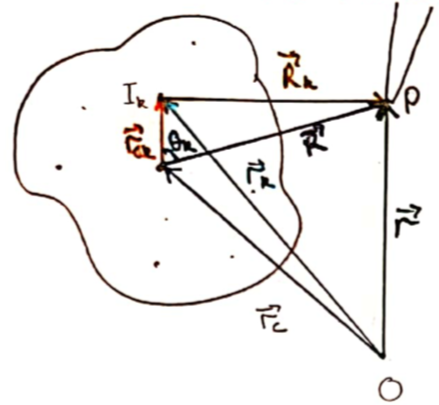
\includegraphics[width=0.3\textwidth]{Figures/placeholder_appB1.png}
	\end{center}
	\caption{\textbf{Placeholder: Electric potential from volume containing current sinks and sources}}
	\label{fig:current_volume}
\end{figure}

Our first step is to write $\frac{1}{|{\bf r} - {\bf r}_k|} = \frac{1}{R_k}$ from \fref{eq:point_source} as an infinite series. Here, $R_k$ is the distance between current $I_k$ at ${\bf r}_k$ and the electrode position ${\bf r}$.

We start by applying the cosine rule,
\begin{equation}\label{eq:cos}
R_k^2 = R^2 + r_{ck}^2 - 2 R r_{ck} \cos \theta_k.
\end{equation}
where $r_{ck} = |{\bf r}_{ck}|$ is the length of the distance vector between the volume mid point ${\bf r}_c$ and current location ${\bf r}_k$, and $\theta_k$ is the angle between ${\bf r}_{ck}$ and ${\bf R}$, see \fref{fig:theta_k}.

\begin{figure}[!ht]
	\begin{center}
		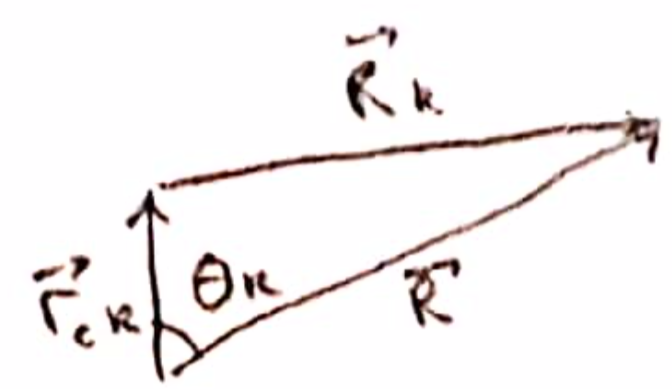
\includegraphics[width=0.3\textwidth]{Figures/placeholder_appB2.png}
	\end{center}
	\caption{\textbf{Placeholder: Angle between ${\bf r}_{ck}$ and ${\bf R}$}}
	\label{fig:theta_k}
\end{figure}

Further, we rewrite \fref{eq:cos} above to get the following expression for $R_k$:

\begin{align*}
R_k^2 &= R^2\big[1 -  \frac{r_{ck}}{R} 2 \cos \theta_k + \big(\frac{r_{ck}}{R}\big)^2  \big] \\
\implies R_k &= R\sqrt{1 - 2 h \cos \theta_k + h^2} \quad \forall h = \frac{r_{ck}}{R}
\end{align*}

%
This means that we can write:

\begin{equation*}
\frac{1}{|{\bf r} - {\bf r}_k|} = \frac{1}{R\sqrt{1 - 2 h \cos \theta_k + h^2}}
\end{equation*}

Noticing that $\frac{1}{\sqrt{1 - 2 h \cos \theta_k + h^2}}$ is the generating function for the Legendre polynomials, we find that

\begin{align*}\label{eq:legendre}
\frac{1}{\sqrt{1 - 2h\cos \theta_k + h^2}} &= \sum_{l = 0}^\infty h^l P_l(\cos \theta_k) \quad \quad \quad \forall \quad |h| = |\frac{r_{ck}}{R}| < 1 \\
\implies \frac{1}{|{\bf r} - {\bf r}_k|} &= \frac{1}{R} \sum_{l = 0}^\infty \big(\frac{r_{ck}}{R}\big)^l P_l(\cos \theta_k) \quad \quad \forall \quad R > r_{ck}.
\end{align*}
Here, $P_l$  are the Legendre polynomials, such that:
\begin{align*}
P_0 (\cos \theta_k) &= 1 \\
P_1 (\cos \theta_k) &= \cos \theta_k \\
P_2 (\cos \theta_k) &= \frac{3}{2} \cos^2 \theta_k - \frac{1}{2} \\
P_3 (\cos \theta_k) &= \frac{5}{2} \cos^3 \theta_k - \frac{3}{2}\cos \theta_k \\
&\;\;\vdots \notag
\end{align*}

Inserting our infinite series expression for $\frac{1}{|{\bf r} - {\bf r}_k|}$ into \fref{eq:point_source}, we arrive at the current multipole expansion:

\begin{equation}\label{eq:multipole_compact}
\Phi (R) = \frac{1}{4 \pi \sigma}\frac{1}{R} \sum_{k=1}^N I_k \sum_{l = 0}^\infty \big(\frac{r_{ck}}{R}\big)^l P_l(\cos \theta_k) \quad \forall~ R > r_{ck}.
\end{equation}

Writing out the first terms, we find that

\begin{align}\label{eq:multipole}
\Phi(R) =~& 
\frac{1}{4 \pi \sigma} \Bigg[\frac{1}{R} \sum_{k=1}^N I_k \nonumber\\
&~~~~+ \frac{1}{R^2} \sum_{k=1}^N I_k r_{ck} \cos \theta_k \\
&~~~~+  \frac{1}{R^3} \sum_{k=1}^N I_k r_{ck}^2 \left( \frac{3}{2} \cos^2 \theta_k - \frac{1}{2} \right) \nonumber \\
&~~~ +  \frac{1}{R^3} \sum_{k=1}^N I_k r_{ck}^3 \left( \frac{5}{2} \cos^3 \theta_k - \frac{3}{2} \cos \theta_k \right) ... \nonumber \Bigg] \quad \forall R > r_{ck}.
\end{align}

Here, the first four terms are known as the monopole $\Phi^{\mathrm{mono}}$, dipole $\Phi^{\mathrm{dipole}}$, quadrupole $\Phi^{\mathrm{quadrupole}}$ and octopole $\Phi^{\mathrm{octopole}}$ contributions, respectively, such that

\begin{equation}
\Phi = \Phi^{\mathrm{monopole}} + \Phi^{\mathrm{dipole}} + \Phi^{\mathrm{quadrupole}} + \Phi^{\mathrm{octopole}} + ...
\end{equation}

Now, we are going to take a look at how the first four terms of the current multipole expansion contribute to the extracellular potential in neural tissue.

\section{Monopole contribution in neural tissue}\label{sec:mono}
Due to current conservation in neural tissue, the transmembrane current sinks and sources for a whole number of neurons will always sum to zero: $\sum_k I_k = 0$. This means that the monopole contribution term will always be zero in neural tissue:

\begin{equation*}
\Phi^{\mathrm{monopole}} = \frac{1}{4 \pi \sigma} \frac{1}{R} \sum_k I_k = 0
\end{equation*}

\section{Dipole contribution in neural tissue/ the current dipole approximation}
The dipole contribution is given as 
\begin{equation*}
\Phi^{\mathrm{dipole}} = \frac{1}{4 \pi \sigma} \frac{1}{R^2} \sum_k I_k r_{ck} \cos \theta_k
\end{equation*}
Applying the definition of the scalar product ${\bf r}_{ck} \cdot {\bf R} = r_{ck} \text{R} \cos \theta_k$, we see that $r_{ck} \cos \theta_k = {\bf r}_{ck} \cdot {\bf \hat{R}}$, where $\hat{{\bf R}} = {\bf R}/\text{R}$ , we can write the expression above as follows:

\begin{align*}
\Phi^{\mathrm{dipole}} &= \frac{1}{4 \pi \sigma} \frac{1}{R^2} \sum_k I_k {\bf r}_{ck} \cdot {\bf \hat{R}} \\
		   &= \frac{1}{4 \pi \sigma} \frac{1}{R^2} \sum_k I_k ({\bf r}_{k} - {\bf r}_{c}) \cdot {\bf \hat{R}} \\
 		   &= \frac{1}{4 \pi \sigma} \frac{1}{R^2} \left(\sum_k I_k {\bf r}_{k} \cdot {\bf \hat{R}} - \sum_k I_k {\bf r}_{c} \cdot {\bf \hat{R}} \right)
\end{align*}
Since $\sum_k I_k {\bf r}_k = {\bf p}$ and $\sum_k I_k = 0$, we here end up with the current dipole approximation:

\begin{equation}
\Phi \approx \Phi^{\mathrm{dipole}} = \frac{1}{4 \pi \sigma} \frac{{\bf p} \cdot {\bf \hat{R}}}{\text{R}^2} = \frac{1}{4 \pi \sigma} \frac{\text{p} \cos \theta}{R^2},
\end{equation}

Here, $\theta$ is the angle between ${\bf p}$ and ${\bf R}$. Since the current dipole approximation is based on the multipole expansion, the constraint $\text{R} > r_{ck}$ still holds.

In \fref{sec:mono}, we saw that there are no monopole contributions to electric potentials from a whole number of neurons. However, applying the current-dipole approximation, we neglect the higher-order terms in the current multipole expansion, which calls for stricter constraints: $R >> r_ck$. In order to get an intuition about when $R$ is "large enough", we will look into the quadrupole and octopole contributions ($\Phi^{\mathrm{quadrupole}}$, $\Phi^{\mathrm{octopole}}$) from a single current sink and a current source.

\section{Quadrupole contribution from a single current sink source pair}\label{sec:quad}

From \fref{eq:multipole}, we see that the quadrupole contribution for a current sink $I_1$ at $r_1$ and a current source $I_2$ at $r_2$ is

\begin{equation}\label{eq:phi_quad}
\Phi^{\mathrm{quadrupole}} = \frac{1}{R^3} \left[ I_1 r_{c1}^2 \left( \frac{3}{2} \cos^2 \theta_1 - \frac{1}{2} \right) + I_2 r_{c2}^2 \left( \frac{3}{2} \cos^2 \theta_2 - \frac{1}{2} \right) \right].
\end{equation}

When the center of the volume is defined halfway between the sink and the source $I_2 = -I_1$, we know that $r_{c1} = r_{c2}$, and that

\begin{align*}
\theta_2 &= \pi - \theta_1 \\
\implies \cos \theta_2 &= -\cos \theta_1 \\
\implies \cos^2 \theta_2 &= \cos^2 \theta_1.
\end{align*}

Inserting this into \fref{eq:phi_quad}, we see that $\Phi^{\mathrm{quadrupole}} = 0$, meaning that there is no quadrupole contribution to the extracellular potential from a sink-source pair.

Since all terms of Legendre polynomials for $l = 4, 6, 8, ...$ contain $\cos \theta_k$ raised to the power of an even number, multipole expansion term number 3, 5, 7, 9, etc are all equal zero for a sink-source pair.

\section{Octopole contribution from a single current sink source pair}\label{sec:octo}

For a sink-source current pair, $I_1$ at ${\bf r}_1$ and $I_2$ at ${\bf r}_2$, we have the following octopole contribution:

\begin{equation*}
\Phi^{\mathrm{octopole}} = \frac{1}{4 \pi \sigma} \frac{1}{R^4}\left[ 
I r_{c1}^3 \left( \frac{5}{2} \cos^3 \theta_1 - 
\frac{3}{2}\cos \theta_1 \right) - 
I r_{c2}^3 \left( \frac{5}{2} \cos^3 \theta_2
 - \frac{3}{2} \cos \theta_2 \right)
\right].
\end{equation*}

If ${\bf r}_{c}$ is the midpoint between ${\bf r}_1$ and ${\bf r}_2$, we can say that $r_{c2} = r_{c1} = \frac{d}{2}$ and $\cos \theta_2 = - \cos \theta_1$. This implies that

\begin{align*}
\Phi^{\mathrm{octopole}} &= \frac{1}{4 \pi \sigma} \left[
I \frac{d}{2}^3 \left( \frac{5}{2} \cos^3 \theta_1 - 
\frac{3}{2}\cos \theta_1 \right) - 
I \frac{d}{2}^3 \left( \frac{5}{2} \cos^3 \theta_1
 - \frac{3}{2} \cos \theta_1 \right)
\right] \\
&= \frac{1}{4 \pi \sigma} \frac{I d^3}{R^4} \frac{1}{16} \left(
5 \cos^3 \theta_1 - 3 \cos \theta_1 + 5 \cos^3 \theta_1 - 3 \cos \theta_1
\right) \\
&= \frac{1}{4 \pi \sigma} \frac{I d^3}{R^4} \frac{5 \cos^3 \theta_1 - 3 \cos \theta_1}{8}
\end{align*}

For a single current sink source pair $\theta_1 = \theta$, where $\theta$ is the angle between ${\bf p}$ and ${\bf R}$, such that

\begin{align*}
\Phi^{\mathrm{octopole}} = \frac{1}{4 \pi \sigma} \frac{p}{R^2} \frac{d^2}{R^2} \frac{5 \cos^3 \theta - 3 \cos \theta}{8}.
\end{align*}

Including the octopole contribution when estimating the extracellular potential from a sink-source pair, as opposed to applying the current dipole approximation, can be quantified as follows:

\begin{equation*}
\big| \frac{\Phi^{\mathrm{octopole}}}{\Phi^{\mathrm{quad}}} \big|_{\mathrm{max}} = \big|\frac{d^2}{R^2} \frac{5 \cos^2 \theta - 3}{8}\big|_{\mathrm{max}} = \frac{3}{8} \frac{d^2}{R^2}
\end{equation*}

In \citeasnoun**{Nunez2006}, it is suggested that the current dipole approximation is applicable when $R > 3d$ or $R > 4d$.

For a sink-source pair, the octopole contribution is maximum $\Phi^{\mathrm{octo}}(R = 3d) = \frac{1}{24} \Phi^{\mathrm{dipole}}$ and $\Phi^{\mathrm{octo}}(R = 4d) = \frac{3}{128} \Phi^{\mathrm{dipole}}$.

%\snnote{current dipole approximation, suggestion 2}
%\slntxt{  
%	
%	In the next paragraph, we outline the current dipole approximation, as an alternative to eq.~\eqref{eq:VCtheory}. We picture $N$ currents $I_k$ located at $\mathbf{r}_k$ in a volume centered around position $\mathbf{r}_c = \sum_{k = 1}^N \frac{\mathbf{r}_k}{N}$. Our measurement electrode is positioned a distance $R = |\mathbf{R}| = |\mathbf{r}_c - \mathbf{r}|$ away from the current distribution.
%	
%	Starting out with eq.~\eqref{eq:VCtheory}, we can rewrite $\frac{1}{|\mathbf{r} - \mathbf{r}_k|}$ as a binomial expansion, by first applying the cosine rule. From this, we end up with an infinite series, better known as the multipole expansion for current sources:
%	
%	\begin{align}\label{eq:multipole}
%	\Phi(R) =~& 
%	\frac{1}{4 \pi \sigma} \Bigg[\frac{1}{R} \sum_{k=1}^N I_k \nonumber\\
%	&~~~~+ \frac{1}{R^2} \sum_{k=1}^N I_k r_k^c \cos \theta_k \\
%	&~~~~+  \frac{1}{R^3} \sum_{k=1}^N I_k r_k^{c~2} \left( \frac{3}{2} \cos^2 \theta_k - \frac{1}{2} \right) + ... \nonumber \Bigg]
%	\end{align}
%	
%	Where $r_k^c = |\mathbf{r}_k^c|$ is the distance between current source $k$ at position $\mathbf{r}_k$ and the distribution midpoint $\mathbf{r}_c$,
%	and $\theta_k$ is the angle between $\mathbf{r}_k^c$ and $\mathbf{R}$.
%	The multipole expansion gives us the exact potential at location $\mathbf{r}$, when $R > r_{k~max}$. Computing electric potentials applying the multipole expansion directly, is however not very useful, since we would need infinitely many terms.
%	Looking at the various terms in the multipole expansion, we notice that the terms decay with distance from the current distribution as $1/R$, $1/R^2$, $1/R^3$. The terms are often referred to as the \emph{monopole contribution}, the \emph{dipole contribution}, the \emph{quadrupole contribution}, etc, respectively.  For the case of a single current source, all terms but the monopole contribution, would give non-zero contributions to the electric potential. Due to current conservation, single current monopoles are unphysical in neural tissue.
%	The simplest current distribution that can result from neural activity is the current dipole, i.e. a current sink $I_1 = -I$ and a current source $I_2 = I$. Inserting this into the multipole expansion, we see that there is no monopole contribution, but the dipole contribution and higher-order terms will  contribute to the electric potential.
%	The dipole contribution from a single current dipole is known as the current dipole approximation and can be written on the form:
%	\begin{equation}\label{eq:CDA}
%	\Phi^{dipole}(\mathbf{R}) = \frac{1}{4 \pi \sigma} \frac{|\mathbf{p}| \cos \theta}{R^2},
%	\end{equation}
%	where $R = |\mathbf{r}_c - \mathbf{r}|$ is the distance from the midpoint of the so-called current dipole moment $\mathbf{p}$ to the electrode, and $\theta$ is the angle between $\mathbf{p}$ and $\mathbf{R}$.
%	
%	The current dipole moment from a current sink $I_1 = I$ and a current source $I_2 = -I$, located at position $\mathbf{r}_1$ and $\mathbf{r}_2$, respectively, can be calculated as
%\begin{align}\label{eq:p}
%\mathbf{p} &= I_1 \mathbf{r}_1 + I_2 \mathbf{r}_2 \nonumber\\
%&= I \mathbf{r}_1 - I \mathbf{r}_2 \\
%&= I \mathbf{d}, \nonumber
%\end{align}
%	
%	where $\mathbf{d}$ is the distance vector between the current sink and the current source, giving the length and direction of the dipole.
%	
%	Applying the current dipole approximation, we neglect the quadrupole and higher-order contributions to the electric potential. This is a good approximation in the far-field limit, that is when $R$ is much larger than the dipole length $d$, $R > 3d$ or $R > 4d$, since the higher-order terms decay rapidly with increasing distance \cite**{Nunez2006}.
%}
%
%\snnote{To be included for both suggestions:}
%
%\sntxt{
%	
%	It is important to note that when computing the electric potential in the far-field limit from a distribution of transmembrane currents in neural tissue, the dipole contribution will be the dominating term \cite**{Nunez2006}. By computing the total current dipole moment from a distribution of current sources
%	\begin{equation}
%	\mathbf{p} = \sum_{k=1}^N I_k \mathbf{r}_k,
%	\end{equation}
%	
%	we can approximate the electric potential from neural activity by applying the current dipole approximation.
%	
%	The point-source approximation, eq. \ref{eq:VCtheory} (or the line-source version of it), and the current dipole approximation, eq.~\eqref{eq:CDA} represent} volume conductor theory in its simplest form, and \sntxt{are} based on a set of assumptions, some of which may be relaxed for problems where it is relevant: 
%\section{Synapses \Comment{- Gaute}}
%\subsection{Chemical synapses:  postsynaptic response}
%\subsection{Chemical synapses:  synaptic plasticity}
%\subsection{Electrical synapses: gap junctions}
\section*{References}
\bibliography{ECS_book.bib}
%\section*{Index}
\printindex
\end{document}

